\documentclass{article}

\usepackage[T2A]{fontenc}
\usepackage[utf8]{inputenc}
\usepackage[russian]{babel}
\usepackage{commath}
\usepackage{amsmath}
\usepackage{amsfonts}
\usepackage{mathtools}
\usepackage{amssymb} 
\usepackage{parskip}
\usepackage{titling}
\usepackage{color}
\usepackage{hyperref}
\usepackage{cancel}
\usepackage{enumerate}
\usepackage{graphicx}
\usepackage[a4paper, left=2.5cm, right=1.5cm, top=2.5cm, bottom=2.5cm]{geometry}

\graphicspath{ {./images/} }
\setlength{\droptitle}{-3cm}
\hypersetup{
    colorlinks=true, %set true if you want colored links
    linktoc=all,     %set to all if you want both sections and subsections linked
    linkcolor=blue,  %choose some color if you want links to stand out
}

\pagenumbering{arabic}

\begin{document}
\title{Летняя сессия по математике}
    \begin{titlepage}
        \begin{center}
            \vspace*{1cm}
                
            \Huge
            \textbf{Математика 2-й семестр, 10-й класс}
                
            \vspace{5cm}
            
            \Large
            \textbf{Ученики 10-4 класса}\\
            \textbf{Оконешников Д.Д., Паньков М.А. и Кангелдиева А.С.}\\
            \textbf{по лекциям к.ф.-м.н. Протопоповой Т.В.}

            \vfill

            \vspace{0.8cm}

            \Large
            
            Для внутреннего использования
            
            Россия, г. Новосибирск, СУНЦ НГУ, 2021 год
            
            v1.4.0
                
        \end{center}
    \end{titlepage}
    \newpage
    % \author{Ученики 10-4 класса Оконешников Д.Д., Паньков М.А. и Кангелдиева А.С. \\по лекции к.ф.-м.н. Протопоповой Т.В.}
    % \date{от 18 мая 2021 г.}
    % \maketitle
	
    \tableofcontents
	\thispagestyle{empty}
	\setcounter{tocdepth}{5}
	\newpage
    
    \section{Элементы теории чисел}
    	\subsection{Определение операции деления с остатком для целых чисел.}
    		\textbf{Определение.} Для \( a \in \mathbb{Z} \) и \( b \in \mathbb{Z} \backslash \{0\} \) определена операция деления с остатком: разделить целое \( a \) на целое \(b\ (\neq 0) \) с остатком, 
			означает найти такие целые \( q,\ r \in \mathbb{Z} \), что \(a=b*q+r,\ 0 \leq r < \abs{b} \).
            
  			\textbf{Определение.} Если при делении с остатком \( r = 0 \), то число \( a \) делится на \( b\ (a \vdots b) \). Число \( b \) при этом называется делителем числа \( a \).	
            
        \subsection{Свойства делимости}
        	\begin{tabular}{ll}
            \textbf{(1)} Если \( a \vdots c \) и \(b \vdots c\), то \( (a \pm b) \vdots c \) & \textbf{(5)} \( a \vdots b \) и \( b \vdots a \Rightarrow \abs{a} = \abs{b} \)\\
            \( \uparrow
              \begin{aligned}
                &a = cq_1\\
                &b = cq_2
              \end{aligned}
            \Rightarrow (a \pm b) = c(q_1 \pm q_2) \Rightarrow (a \pm b) \vdots c \downarrow \) & \textbf{(6)} \( \forall\ a \in \mathbb{Z} \backslash \{0\} \Rightarrow 0 \vdots a \)\\
            \textbf{(2)} \( a \vdots b \Rightarrow ak \vdots b\ (k \in \mathbb{Z})\) & \textbf{(7)} \( \forall\ a \in \mathbb{Z} \Rightarrow a \vdots 1 \)\\
            \textbf{(3)} \( a \vdots b,\ b \vdots c \Rightarrow a \vdots c \) & \textbf{(8)} Если \( ab \vdots m \) и \( \textrm{НОД}(a,\ m) = 1, \textrm{ то } b \vdots m \)\\
            \( \uparrow a = bq_1,\ b=cq_2 \Rightarrow a = c*(q_1*q_2) \Rightarrow a \vdots c \downarrow \) & \textbf{(9)} Если \(a \vdots m,\ a \vdots k \textrm{ и НОД}(m,\ k) = 1, \textrm{ то } a \vdots mk \)\\
            \textbf{(4)} Если \( a \neq 0,\ a \vdots b \Rightarrow \abs{a} \geq \abs{b} \) &\\
            \( \uparrow a \vdots b \Leftrightarrow a = b*q \Rightarrow \abs{a} = \abs{b} * \abs{q} \Rightarrow \) от противного, &\\
            если \( \abs{a} < \abs{b} \), то \( \abs{q} = \frac{\abs{a}}{\abs{b}} < \frac{\abs{b}}{\abs{b}} = 1 \Rightarrow \) единственная &\\
            возможность при целом \( q:\ q = 0 \), но тогда и \( a = 0 \).&\\
            Противоречие. \( \downarrow \) &\\
          \end{tabular}
          
  	    \subsection{Простые и составные числа}
        	\textbf{Определение.} Натуральное число \( p > 1 \) называется простым, если оно имеет ровно два натуральных делителя \( (p \textrm{ и } 1) \).

  			Все остальные натуральные числа называются составными (кроме 1). Единица не является ни простым, ни составным.
            
        \subsection{Основная теорема арифметики}
        	\textbf{Теорема.} Всякое натуральное число \( n > 1 \) может быть представлено в виде \( n = p_1*p_2* ... *p_i \), где \( p_i \) --- простые числа. Это представление единственно с точностью до порядка множителей (т.е. если \( n = p_1*p_2*...*p_r = q_1*q_2*...*q_s \), то \( r = s \) и \(q_1,\ q_2,...,\ q_s \) можно перестановкой получить из чисел \( p_1,\ p_2,...,\ p_r \)).

            \textbf{(1)} \underline{Докажем существование} 

            Пусть \(n \in \mathbb{N},\ n > 1 \). Среди делителей \( n \) есть числа превосходящие 1 (например, само \( n \)). Пусть \( p_1 \) --- наименьший из таких делителей.

            \( p_1 \) --- простое число (если оно само имело бы делитель \(a:\ 1 < a < p_1 \), то \( a \) было бы меньше \( p_1 \) и было бы делителем \( n \) (св-ва 4,3), противоречит тому, что выбран наименьший делитель).

            Итак, \( n = p_1n_1, \textrm{ где } p_1 \textrm{ --- простое, } n_1 \in \mathbb{N} \textrm{ и } n_1 < n \) (св-во 4).

            Если \( n_1 > 1 \), то поступим с ним так же, как и числом \( n \), представим его в виде \( n_1 = p_2n_2 \), \( p_2 \) --- простое, \( n_2 \in \mathbb{N}, n_2 < n_1 \Rightarrow n = p_1*p_2*n_2 \) и т.д.

            В конце концов, так как \( n_i \in \mathbb{N}, i=1,2,3,... \) убывают, то \( \exists\ n_r = 1 \) и процесс обрывается: \( n=p_1*p_2*...*p_r \)

            \textbf{(2)} \underline{Докажем единственность}
            
            От противного. Если \( \exists \) хоть одно натуральное число, допускающее два существенно различных разложения, то непременно \( \exists \) и \underline{наименьшее} число с таким свойством: \[ m = p_1*p_2*...*p_r = q_1*q_2*...*q_s \qquad (1) \]
            Можем допустить, что \( p_1 \leq p_2 \leq ... \leq p_r;\ q_1 \leq q_2 \leq ... \leq q_s \).

            А) Заметим, что \( p_1 \neq q_1 \).\\
            Если равны, то разделив (1) на \( p_1 = q_1 \), получили бы два существенно различных разложения на простые множители для числа \( < m \) (Противоречие с тем, что \( m \) --- наименьшее).\\
            На самом деле показали больше: что среди \( q_j \) нет чисел равных какому-либо \( p_i \)

            Б) Из А) \( p_1 < q_1 \) или \( p_1 > q_1 \). Пусть \( p_1 < q_1 \) (для \( p_1 > q_1 \) доказательство строится аналогично).\\
            Рассмотрим целое число: \[ m' = m - p_1*q_2*...*q_s\qquad (2) \]
            Подставляя вместо \( m \) два его разложения, получим: \[ m' = p_1*p_2*...*p_r - p_1*q_2*...*q_s = p_1(p_2*...*p_r - q_2*...*q_s)\qquad (3) \] \[ m' = q_1*q_2*...*q_s - p_1*q_2*...*q_s = (q_1 - p_1)q_2*...*q_s\qquad (4) \]
            Из равенства (4) очевидно \( m' > 0 \). Из равенства (2) \( m' < m \), а значит, для \( m' \) разложение на простые множители --- единственно (с точностью до порядка сомножителей).

            Из (3) \( \Rightarrow p_1 \) входит множителем в \( m' \), значит, из (4) \( p_1 \) входит множителем либо в \( q_1 - p_1 \), либо в \( q_2*...*q_s \). Но последнее невозможно, так как все \( q_j > p_1\ (p_1 < q_1) \) и они простые.

            Значит, \( p_1 \) входит множителем в \( q_1 - p_1 \), т.е. \( \mathbf{(q_1 - p_1) \vdots p_1} \) \( \Rightarrow q_1 - p_1 = p_1h \Rightarrow q_1 = p_1(h + 1) \), т.е. \( \mathbf{q_1 \vdots p_1} \), чего быть не может. Противоречие. Ч.Т.Д.
            
        \subsection{Теорема о количестве простых чисел (Теорема Евклида)}
            \textbf{Теорема.} Множество простых чисел бесконечно.

            \( \uparrow \) Доказательство проведем от противного. Предположим, что множество простых чисел конечно, т.е. \( P=\{p_1,p_2,...,p_k\} \) --- конечная совокупность простых чисел.

            Рассмотрим число \( p = p_1*p_2*...*p_k + 1 \).

            Заметим, что \( \forall\ i,\ i=1,2,...,k \) это \( p > p_i \), т.е. \( p \notin P \), значит, оно составное и по ОТА может быть представлено в виде произведения простых множителей.

            Но \( p \) не делится ни на какой \( p_i \) (при делении дает в остатке 1).

            Значит, наше предположение о конечности системы простых чисел неверно. \( \downarrow \)
            
        \subsection{Как часто встречаются простые числа на числовой оси? (утверждение)} 
        	\textbf{Утверждение.} Существуют сколь угодно длинные участки натурального ряда, вовсе не содержащие простых чисел

            \( \uparrow \) Действительно, пусть \( n \in \mathbb{N}, n > 1 \). Рассмотрим ряд чисел: \( n! + 2,n! + 3,...,n! + n \).

            \begin{tabular}{ll}
              \( n = 2: 2! + 2 \) --- одно число в ряду; &\\
              \( n = 3: 3! + 2, 3! + 3 \) --- два числа в ряду; & чем больше \( n \), тем больше в ряду\\
              \( n = 4: 4! + 2, 4! + 3, 4! + 4 \) --- три числа в ряду; & чисел (\( n - 1 \) число).\\
              и т.д. &\\
            \end{tabular}

            В этом ряду нет ни одного простого числа, так как \( n! + 2 \) делится на 2, \( n! + 3 \) делится на 3, \( n! + n \) делится на n. Таким образом, при больших \( n \) такие участки натурального ряда могут быть очень большими. \( \downarrow \) 
            
        \subsection{Теорема Эйлера}
            \textbf{Теорема.} Пусть \( \tau(n) \) --- количество простых чисел \( \leq n \). Тогда \[ \frac{\tau(n)}{n} \xrightarrow[n \rightarrow \infty]{} 0 \]
            Понятно, что \( \tau(n) \) увеличивается (т.е. \( \rightarrow \infty \)) при \( n \rightarrow \infty \) (это означает, что простые числа встречаются все реже и реже).

        \subsection{Каноническое разложение, число всех натуральных делителей натурального числа}
            Мы показали, что любое натуральное число мы можем представить в виде произведения простых множителей (и такое представление единственно с точностью до перестановки множителей): \( n = p_1*p_2*...*p_r,\ p_1 \leq p_2 \leq ... \leq p_r \). Используя обозначение степени, можем записать так:
            \[ \mathbf{n = p_1^{a_1}*p_2^{a_2}*...*p_k^{a_k}}, \textrm{ (каноническое разложение) } \] 
            \[ \textrm{где } p_1 < p_2 < ... < p_k \textrm{ --- простые, } a_1, a_2, ..., a_k \textrm{ --- натуральные числа.} \]
            \textbf{Замечание.} Бывает полезно записать в разложение \underline{все} простые числа \( \leq p_k \) и использовать показатель равный 0.

            Если число \( m \) является делителем \( n \), то несложно понять, что \( \mathbf{m = p_1^{\beta_1}*p_2^{\beta_2}*...*p_k^{\beta_k}} \), где \( 0 \leq \beta_i \leq a_i \).

            Можно посчитать число всех натуральных делителей числа \( n \). Любой делитель \( n \) имеет следующую структуру: \( \mathbf{m = p_1^{0,1,2,...,a_1}*p_2^{0,1,...,a_2}*...*p_k^{0,1,...,a_k}} \)

            Для первого множителя \( (a_1 + 1) \) возможность для второго \( (a_2 + 1) \) возможностей и т.д. Таким образом, число всех делителей \( (a_1 + 1)*(a_2 + 1)*...*(a_k + 1) \).

            \textbf{Пример.} Сколько делителей у числа 120 (включая 1 и само число)?

            \begin{tabular}{r|l}
              120 & 2\\
              60 & 2\\
              30 & 2\\
              15 & 3\\
              5 & 5\\
              1 & \\
            \end{tabular}

            \( 120 = 2^3 * 3^1 * 5^1 \). Значит, число всех делителей \( = (3 + 1)*(1 + 1)*(1 + 1) = 4*2*2 = 16 \).

        \subsection{НОД и НОК}
            \textbf{Определение.} \( d \) --- общий делитель \( a \) и \( b \Leftrightarrow \mathbf{a \vdots d } \) и \( \mathbf{b \vdots d} \).

            \textbf{Определение.} Наибольший общий делитель чисел \( a \) и \( b \) обозначается \( \textrm{НОД}(a, b) \).

            \textbf{Определение.} Наименьшее общее кратное \( \textrm{НОК}(a, b) = k \) --- наименьшее натуральное число такое, что \( \mathbf{k \vdots a} \) и \( \mathbf{k \vdots b} \).

            Пусть \( \mathbf{a = p_1^{a_1} * p_2^{a_2} * ... * p_k^{a_k}},\ \mathbf{b = p_1^{\beta_1} * p_2^{\beta_2} * ... * p_k^{\beta_k}} \)

            Здесь использовали показатель 0 для тех простых множителей, которые входят только в одно из разложений.

            Тогда \[ \textrm{НОД}(a, b) = p_1^{min(a_1, \beta_1)} * p_2^{min(a_2, \beta_2)} * ... * p_k^{min(a_k, \beta_k)} \]
            \[ \textrm{НОК}(a, b) = p_1^{max(a_1, \beta_1)} * p_2^{max(a_2, \beta_2)} * ... * p_k^{max(a_k, \beta_k)} \]
            \[ \textrm{НОД}(a, b)*\textrm{НОК}(a, b) = a * b \]

            \textbf{Пример.} \( a = 2 * 3^3 * 5^2 * 7,\ b = 2^2 * 3 * 7^2 * 11 \Rightarrow a = 2^1 * 3^3 * 5^2 * 7^1 * 11^0,\ b = 2^2 * 3^1 * 5^0 * 7^2 * 11^1 \Rightarrow \textrm{НОД}(a, b) = 2^1 * 3^1 * 5^0 * 7^1 * 11^0,\ \textrm{НОК}(a, b) = 2^2 * 3^3 * 5^2 * 7^2 * 11^1 \).

        \subsection{Доказательство свойств делимости 8 и 9}
            \textbf{Свойство 8.} Если \( ab \vdots m \) и \( \textrm{НОД}(a, m) = 1 \), то \( b \vdots m \)

            \( \uparrow \) Имеем \( \textrm{НОД}(a,m) = 1 \Rightarrow \exists A,\ M: Aa + Mm = 1. \)\\
            Домножим последнее равенство на \( b: \underset{\vdots m}{Aab} + \underset{\vdots m}{Mmb} = b \Rightarrow b \vdots m \downarrow \)

            \textbf{Свойство 9.} Если \( a \vdots m,\ a \vdots k \) и \( \textrm{НОД}(m,k) = 1 \), то \(a \vdots mk \)

            \( \uparrow \)

            1) \( a \vdots m \Rightarrow a = mq_1 \)\\
            2) \( a \vdots k \Rightarrow mq_1 \vdots k \)\\
            3) из 2) и \( \textrm{НОД}(m,k) = 1 \Rightarrow \) по свойству 8 \( q_1 \vdots k \Rightarrow q_1 = kq_2 \)\\
            4) \( a = mq_1 = mkq_2 \), т.е. \( a \vdots mk \downarrow \)
            
        \subsection{Признаки делимости на 2, 3, 4, 5, 6, 8, 9, 11}
        	1) на 2 и 5. Легко.\\
            2) на 4. \( n = \overline{a_ka_{k-1}...a_1a_0} = 100 * \overline{a_ka_{k-1}...a_2} + \overline{a_1a_0}.\quad 100 \vdots 4.\ \Rightarrow n \vdots 4 \Leftrightarrow \overline{a_1a_0} \vdots 4 \).\\
            3) на 8. \( n \vdots 8 \Leftrightarrow \overline{a_2a_1a_0} \vdots 8 \).\\
            4) на 3. \( n = \overline{a_ka_{k-1}...a_1a_0} = a_k10^k + a_{k-1}10^{k-1} + ... + a_1 10 + a_0 = a_k(\underbrace{999...9}_k + 1) + a_{k-1}(\underbrace{999...9}_{k-1} + 1) + ... + a_1(9 + 1) + a_0 = (a_k\underbrace{999...9}_k + a_{k-1}\underbrace{999...9}_{k-1} + ... + a_1 9) + (a_k + a_{k-1} + ... + a_1 + a_0) \)\\
            Аналогично для 9.\\
            5) на 6. \( n \vdots 2 \) и \( n \vdots 3 \Rightarrow \) (так как 2 и 3 взаимно просты) \( n \vdots 6 \)\\
            6) на 11. \[ n = \overline{a_ka_{k-1}...a_1a_0} = a_0 + a_1 10 + a_2 100 + a_3 1000 + ... + a_k 10^k = \] 
            \[ = a_0 + a_1(11 - 1) + a_2(99 + 1) + a_3(1001 - 1) + a_4(9999 + 1) + a_5(100001 - 1) + ... + a_k 10^k = \] 
            \[ = (a_0 - a_1 + a_2 - a_3 + a_4 - ...) + (a_1 11 + a_3 1001 + a_5 100001 + ... + a_{2l+1}1\underbrace{00...0}_{2l}1 + ... ) +\]
            \[ + (a_2 99 + a_4 9999 + ... + a_{2m}\underbrace{99...99}_{2m} + ...)\]\\
            А) числа, состоящие из четного числа 9-ок, делятся на 11, т.е. последняя скобка \( \vdots 11 \);\\
            Б) заметим, что \( 1001 = (1100 - 99) \vdots 11,\quad 100001 = (110000 - 9999) \vdots 11,\quad 1\underbrace{00...00}_{2l}1 = (11\underbrace{00...00}_{2l} - \underbrace{99...99}_{2l}) \vdots 11 \).
       
        \subsection{Алгоритм Евклида}
        	Пусть требуется найти НОД\( (a,b) \). Будем считать, что \( \abs{a} > \abs{b} \).

            \textbf{1)} Разделим \( a \) на \( b \) с остатком: \[ a = q_1b + r_1,\ 0 \leq r_1 < \abs{b}\quad (1) \]
            Заметим, что любой делитель пары \( (a,b) \) будет делителем \( r_1 \), а значит пары \( (b,r_1) \). С другой стороны, любой делитель пары \( (b,r_1) \) будет делителем \( a \), а значит пары \( (a,b) \). Таким образом (равенство множеств), множество делителей пары \( (a,b) \) совпадает с множеством делителей пары \( (b,r_1) \), а значит и НОД\( (a,b) \) = НОД\( (b,r_1) \).

            \textbf{2)} Разделим \( b \) на \( r_1 \) с остатком: \[ b = q_2r_1 + r_2,\ 0 \leq r_2 < r_1\quad (2) \]
            При этом получаем, что НОД\( (b,r_1) \) = НОД\( (r_1,r_2) \)

            \textbf{3)} Разделим \( r_1 \) на \( r_2 \) с остатком: \[ r_1 = q_3r_2 + r_3,\ 0 \leq r_3 < r_2\quad (3) \]
            При этом НОД\( (r_1, r_2) \) = НОД\( (r_2, r_3) \).\\
            И т.д.

            Посмотрим на остатки. \( \abs{b} > r_1 > r_2 > r_3 > ... \geq 0 \). Получили строго убывающую последовательность неотрицательных целых чисел. Эта последовательность конечна. Существует \( r_{k+1} = 0 \), т.е.

            \textbf{k+1)} \[ r_{k-1} = q_{k+1}r_k + 0\quad (k+1) \]
            При этом НОД\( (a,b) \) = НОД\( (b,r_1) \) = НОД\( (r_1,r_2) \) = НОД\( (r_2,r_3) \) = ... = НОД\( (r_{k-1},r_k) = r_k \).\\
            Таким образом, НОД\( (a,b) \) равен последнему ненулевому остатку в алгоритме Евклида.

            \textbf{Утверждение.} Если \( d = \textrm{ НОД}(a,b) \), то существуют целые \( A \) и \( B: d = Aa + Bb \).

    		\textbf{Замечание.} Если \( \textrm{НОД}(a,b) = 1 \) (т.е. \( a \) и \( b \) взаимно просты), то существуют целые \( A \) и \( B: 1 = Aa + Bb \).

        \subsection{Применение алгоритма Евклида}
            \begin{tabular}{ll}
              Весь алгоритм: & \textbf{Пример.} НОД(5083,3553)-?\\
              \textbf{1)} \( a = q_1b + r_1,\ 0 \leq r_1 < \abs{b} \) & \( 5083 = 1*3553 + 1530 \)\\
              \textbf{2)} \( b = q_2r_1 + r_2,\ 0 \leq r_2 < \abs{r_1} \) & \( 3553 = 2*1530 + 493 \)\\
              \textbf{3)} \( r_1 = q_3r_2 + r_3,\ 0 \leq r_3 < \abs{r_2} \) & \( 493 = 9*51 + 34 \)\\
              ...& \( 51 = 1*34 + 17 \)\\
              \textbf{k)} \( r_{k-2} = q_kr_{k-1} + r_k \) & \( 34 = 2*17 + 0 \Rightarrow \textrm{НОД}(5083,3553) = 17\)\\
              \textbf{k+1)} \( r_{k-1} = q_{k+1}r_{k} + 0 \) & \\
              \( \textrm{НОД}(a,b) = r_k \) & \\
            \end{tabular}
			
        \subsection{Решение уравнений ax + by = c}
        	\textbf{Определение.} Диофантово уравнение первой степени - уравнение вида \( ax + by = c \), где \( a,b,c,x,y \) --- целые числа.

            Пусть \( \textrm{НОД}(a,b) = d \).
            
            \begin{enumerate}
                \item Если \( c \vdots d \), то делим на \( d \) правую и левую части уравнения и получаем \( a_1x + b_1y = c_1 \), где \( \textrm{НОД}(a_1, b_1) = 1 \).\\
                Доказательство следует из очевидного факта, что линейная комбинация двух чисел по-прежнему должна делиться на их общий делитель.
                \item Если \( c \) не делится на \( d \), то уравнение решений не имеет.
            \end{enumerate}

            Таким образом, будем рассматривать уравнения (*) \( ax + by = c,\ \textrm{НОД}(a,b) = 1 \).

            Так как \( \textrm{НОД}(a, b) = 1 \), то по следствию из алгоритма Евклида \( \exists \) целые \( A,\ B: Aa + Bb = 1 \).

            Домножим равенство на \( c: Aca + Bcb = c \).
            
            Видим, что пара целых чисел \( (x_0,y_0) = (Ac, Bc) \) является решением уравнения.

            Мы нашли частное (одно из) решение нашего уравнения. Найдем все решения \( (x,y) \).

            \[ \begin{cases}
                ax_0 + by_0 = c,\\
                ax + by = c.
            \end{cases} \Rightarrow a(x - x_0) + b(y - y_0) = 0,\ a(x - x_0) = -b(y - y_0) \]
            \( \textrm{НОД}(a,b) = 1 \), значит \( (x - x_0) \vdots b \), т.е. \( x - x_0 = bt \) или \( x = x_0 + bt \), где \( t \) --- целое.\\
            Тогда \( y - y_0 = \frac{-a(x - x_0)}{b} = -at \) или \( y = y_0 - at \).\\
            Таким образом, все пары вида \( (x_0 + bt, y_0 - at) \), где \( t \) --- целое, являются решениями (*).

            \textbf{Замечание.} Общее решение диофантова уравнения представляет собой сумму частного решения уравнения и решения соответствующего однородного уравнения (уравнения \( ax + by = 0 \)).

            Легко понять, что решениями однородного уравнения являются все пары вида \( (bt, -at) \), где \( t \) --- целое.

            \textbf{Пример.} 7x - 23y = 131
            
            Проверка решения: \( c\ \vdots \ \textrm{НОД}(a,b) \Rightarrow \) имеет решения.\\ 
            Можно угадать частное решение (22,1), так как 154 - 23 = 131.\\
            Тогда все решения --- \( (22-23t,1-7t),\ t \in \mathbb{Z} \).

        \subsection{Сравнения и их свойства}
        	Основная идея теории сравнений заключается в том, что два числа \( a \) и \( b\ (\in \mathbb{Z}) \), имеющие при делении на \( m \in \mathbb{N} \) один и тот же остаток, обнаруживают целый ряд одинаковых свойств по отношению к \( m \).

            Так по отношению к 2 мы выделяем четные и нечетные числа. Знаем, например, что сумма/разность четных - четное число, произведение четных - четное и т.д.

            \textbf{Определение.} Целые числа \( a \) и \( b \) называются сравнимыми по модулю \( m\ (a \equiv b (mod\ m)) \), если при делении на \( m \) они дают одинаковые остатки. \textbf{(1)}

            \textbf{Пример.} \( 8 \equiv 3 (mod\ 5) \equiv 103 (mod\ 5) \equiv -2 (mod\ 5) \equiv -17 (mod\ 5) \) и т.д.

            \textbf{Определение.} \( a \equiv b (mod\ m) \Leftrightarrow (a - b) \vdots m \). \textbf{(2)}

            Докажем эквивалентность определений 1 и 2.\\
            \( \uparrow \)\\
            1) \textbf{(1)} \( \Rightarrow \) \textbf{(2)}. Пусть остатки одинаковы, т.е. \( a = q_1m + r,\ b = q_2m + r \Rightarrow a - b = m(q_1 - q_2),\ (q_1 - q_2) \in \mathbb{Z} \), т.е. \( (a - b) \vdots m \);\\
            2) \textbf{(2)} \( \Rightarrow \) \textbf{(1)}. От противного.\\
            Пусть остатки разные, т.е. \( a = q_1m + r_1,\ b = q_2m + r_2 \), где \( 0 \leq r_1 < \abs{m},\ 0 \leq r_2 < \abs{m}\ (-\abs{m} < -r_2 \leq 0) \).\\
            Тогда \( a - b = m(q_1 - q_2) + r_1 - r_2 \) и \( -\abs{m} < r_1 - r_2 < \abs{m} (\abs{r_1 - r_2} < \abs{m} \mathbf{(3)}) \Rightarrow (r_1 - r_2) \vdots m \)\\
            Но тогда по свойству делимости 4, если \( r_1 - r_2 \neq 0 \), то \( \abs{r_1 - r_2} \geq \abs{m} \), противоречие с \textbf{(3)}. Таким образом, \(r_1 = r_2. \downarrow \)

            \textbf{Свойства сравнений}
            
            1) \( a \equiv a (mod\ m) \)\\
            2) \( a \equiv b (mod\ m) \Rightarrow b \equiv a (mod\ m) \)\\
            3) \( a \equiv b (mod\ m),\ b \equiv c (mod\ m) \Rightarrow a \equiv c (mod\ m) \)
            \[ \uparrow
                \begin{cases}
                    (a - b) \vdots m,\\
                    (b - c) \vdots m.
                \end{cases} \Rightarrow a - c = \underset{\vdots m}{(a - b)} + \underset{\vdots m}{(b - c)} \vdots m \downarrow \]
            \centerline{Далее считаем, что \( a \equiv b (mod\ m),\ c \equiv d (mod\ m) \)}
            4/5) \( a \pm c \equiv b \pm d (mod\ m) \)
            \[ \uparrow
                \begin{cases}
                    (a - b) \vdots m,\\
                    (c - d) \vdots m.
                \end{cases}
            \Rightarrow (a + c) - (b + d) = \underset{\vdots m}{(a - b)} + \underset{\vdots m}{(c - d)} \vdots m \downarrow \]
            6) \( ac \equiv bd (mod\ m) \) 
            \[ 
                \begin{cases}
                    (a - b) \vdots m,\\
                    (c - d) \vdots m.
                \end{cases}
            \Rightarrow ac - bd = ac - bc + bc - bd = c\underset{\vdots m}{(a - b)} + b\underset{\vdots m}{(c - d)} \vdots m \downarrow \]
            7) \( a^k \equiv b^k (mod\ m) \)\\
            \textbf{Следствие.} Пусть \(P(x)\) --- любой многочлен с целыми коэффициентами, т.е. \(P(x) = a_nx^n + a_{n - 1}x^{n - 1} + ... + a_0\), тогда из \(x \equiv y (mod\ m) \Rightarrow P(x) \equiv P(y) (mod\ m)\).

            8) Если \(ac \equiv bc (mod\ m)\) и \(\textrm{НОД}(c,m) = 1\), то \(a \equiv b (mod\ m)\).\\
            \(\uparrow ac - bc = c(a - b)\). Так как левая часть делится на \(m\) и \(\textrm{НОД}(c,m) = 1\), то \((a - b) \vdots m \downarrow \)\\
            9) Если \(a \equiv b (mod\ m)\) и \(\exists\ k \in \mathbb{Z}: a = ka_1,\ b = kb_1,\ m = km_1\), то \(a_1 \equiv b_1 (mod\ m_1)\).\\
            \( \uparrow a - b = k(a_1 - b_1) \), т.е. \( k(a_1 - b_1) \vdots km_1 \Rightarrow (a_1 - b_1) \vdots m_1 \downarrow \)

            \textbf{Примеры.}

            1) Признак делимости на 3

            \( \forall n \in \mathbb{N}\quad n = a_k10^k + a_{k - 1}10^{k - 1} + ... + a_1 10 + a_0 \). Так как \(10 \equiv 1 (mod\ 3)\), то \(10^k \equiv 1 (mod\ 3) \Rightarrow n(mod\ 3) = (a_k + a_{k - 1} + ... + a_1 + a_0)(mod\ 3)\).

            2) Признак делимости на 11

            Так как \( 10 \equiv -1 (mod\ 11) \), то \( 10^k \equiv (-1)^k(mod\ 11) \).\\
            Тогда \( n(mod\ 11) = ((-1)^ka_k + ... + a_2 - a_1 + a_0)(mod\ 11) \)

            3) Найти остаток от деления на 3 числа \( n = (1^2 + 1)(2^2 + 1)(3^2 + 1)...(1000^2 + 1) \)

            \( n(mod\ 3) = \{(4^2 + 1) = (1^2 + 1)(mod\ 3),\ (4^2 + 1) = (1^2 + 1)(mod\ 3),\ 1000:3 = 333*3 + 1 \} = (1^2 + 1)^{334}(2^2 + 1)^{333}(3^2 + 1)^{333}(mod\ 3) \equiv (2)^{334}(2)^{333}(1)^{333}(mod\ 3) \equiv (2)^{667}(mod\ 3) \equiv (-1)^{667}(mod\ 3) \equiv -1(mod\ 3) \equiv 2(mod\ 3) \).

            4) При каких натуральных \(n\) число \(8n + 3\) делится на 13?

            То есть при каких \(n:\ 8n + 3 \equiv 0(mod\ 13)\)?

            \( 8n \equiv -3(mod\ 13) \)\\
            \( 8n \equiv 10(mod\ 13) \)\\
            \( 4n \equiv 5(mod\ 13) \)\\
            \( 12n \equiv 15(mod\ 13) \)\\
            \( -n \equiv 2(mod\ 13) \)\\
            \( n \equiv -2(mod\ 13) \)\\
            \( n = 13t - 2,\ t \in \mathbb{N} \) или \( n = 13t + 11,\ t \in \mathbb{N} \)

            5) Найти все пары целых чисел \(x\) и \(y\), удовлетворяющих уравнению \(7x - 23y = 131\).

            Избавимся от одного неизвестного: рассмотрим уравнение, например, по модулю 7.

            \( -23y \equiv 131(mod\ 7) \)\\
            \( -2y \equiv 5(mod\ 7) \)\\
            \( 2y \equiv -5(mod\ 7) \)\\
            \( 2y \equiv 2(mod\ 7) \)\\
            \( y \equiv 1(mod\ 7) \Rightarrow y = 7t + 1,\ t \in \mathbb{Z} \)\\
            \( x = \frac{131 + 23y}{7} = \frac{131 + 23*7t + 23}{7} = \frac{154 + 23*7t}{7} = 22 + 23t \)\\
            Ответ: \( (22 + 23t, 1 + 7t), t \in \mathbb{Z} \).
          
        \subsection{Классификация чисел по данному модулю}
        	Поместим все числа сравнимые с данным \(a\) (а значит, сравнимые между собой) по модулю \(m\) в один класс.

            Остатками при делении на \(m\) могут быть \(0,1,2,...,m - 1\).

            Значит, можно выделить ровно \(m\) классов по модулю \(m\).

            Класс характеризуется остатком: \( a = mt + r,\ t \in \mathbb{Z},\ 0 \leq r \leq m - 1 \). Фактически, каждый класс --- арифметическая прогрессия со множителем \(m\).
            
        \subsection{Полная и приведенная системы вычетов}
        	Выберем произвольным образом по одному числу в каждом классе. Такую группу назовем \textit{полной системой вычетов по модулю \(m\ \)}(ПСВ(\(m\))). Для данного \(m\) таких систем существует бесконечно много.

            \textbf{Пример.} По \(mod\ 3\): ПСВ(3) = (0,1,2); ПСВ(3) = (10,11,12); ПСВ(3) = (-4,6,-5).
            
            \textbf{Теорема.} Если $a$ и $m$ взаимно просты, и в выражении $ax + b$ число $x$ пробегает $\textrm{ПСВ}(m)$, то получаемые значения выражения $ax + b$ тоже образуют $\textrm{ПСВ}(m)$.
            
      		$\uparrow$ Так как при $m$ значениях $x$ получаем $m$ значений $ax + b$, то достаточно показать, что все они будут разных классов по $mod\ m$.
            
            От противного: пусть $x_1$ и $x_2$ из разных классов по модулю $m$, а $(ax_1 + b) \equiv (ax_2 + b)(mod\ m) \Rightarrow ax_1 \equiv ax_2(mod\ m)$. Так как $\textrm{НОД}(a,m) = 1$, то $x_1 \equiv x_2(mod\ m)$.
            
            Противоречие. $\downarrow$
            
            \textbf{Следствие.} Рассмотрим $m$ членов арифметической прогрессии 
            \[ b, b + a, b + 2a, ..., b + (m - 1)a, \]
            где $b,a,m \in \mathbb{Z}$ и $\textrm{НОД}(a,m) = 1$. Среди $m$ членов этой арифметической прогрессии имеется ровно один, делящийся на $m$.
            
            $\uparrow$ Заметим, что $(0,1,...,m - 1)$ образуют полную систему вычетов по модулю $m$, но тогда по Теореме эти $m$ членов арифметической прогрессии тоже образуют $\textrm{ПСВ}(m)$, а в ней ровно одно число делится на $m \downarrow$
            
            \textbf{Пример.} Найти все тройки простых чисел вида $p, p + 2, p + 4$
            
            $\uparrow$ Эту тройку чисел можем рассмотреть как 3 последовательных члена арифметической прогрессии с начальным членом $p$ и множителем 2: $p + 0*2, p + 1*2, p + 2*2$.
            
            Так как $\textrm{НОД}(2,3) = 1$, то по следствию к теореме, среди этих трех чисел есть только одно, делящееся на 3. Простое число, делящееся на 3 только 3 $\Rightarrow$
            \[ p = 3 \Rightarrow 3, 5, 7 \textrm{ подходит.},\ p + 2 = 3 \Rightarrow p = 1 \textrm{ не подходит (1 не простое)},\ p + 4 = 3 \Rightarrow \textrm{невозможно} \]
    		
            \textbf{Утверждение.} Все числа, принадлежащие одному классу, имеют с $m$ (в паре) одни и те же общие делители. В том числе один и тот же НОД.
            
            $\uparrow$ Пусть $a$ и $b$ принадлежат одному классу по модулю $m \Rightarrow a = km + r,\ b = lm + r,\ k,l \in \mathbb{Z} \Rightarrow a*b = (k*l)m = qm,\ q \in \mathbb{Z} \Rightarrow a = qm + b$  
            
            Если $d_1$ --- делитель пары $(m, b)$, то $d_2$ --- делитель пары $(m, a)$.
            
            И наоборот, если $d_1$ --- делитель пары $(m, a)$, то $d_2$ --- делитель пары $(m, b)$.
            
            Значит, множество общих делителей пары $(m, a)$ совпадает со множеством общих делителей пары $(m, b)$. Значит и НОД$(m, a) = $ НОД$(m, b) \downarrow$ 
            
            \textbf{Определение.} Группа чисел, содержащая по одному представителю от каждого класса, взаимно простого с модулем, называется приведенной системной вычетов по данному модулю. Обозначение ПрСВ$(m)$
            
            \textbf{Пример.} По модулю 8
            
            ПСВ$(8) = \{1, 2, 3, 4, 5, 6, 7, 8\} \Rightarrow$ ПрСВ$(8) = \{1,3,5,7\} = \{9, -5, 21, -1\}$
            
            \underline{Простейший способ получить ПрСВ(m):} отбираем в ряду чисел $1,2,3,...,m$, представлюящем из себя\\
            ПСВ$(m)$, те, что взаимно просты с $m$.\\
            Таким образом, число классов взаимно простых с $m$, равно числу натуральных чисел $\leq m$ и взаимно простых с $m$. Это число зависит только от $m$ и обозначается $\phi(m)$
        
        	\textbf{Теорема.} Если $a$ и $m$ взаимно просты, и в выражении $ax$ число x пробегает какую-либо ПрСВ$(m)$, то получаемые значения выражения $ax$ тоже образуют ПрСВ$(m)$.
            
            $\uparrow$ Так как одному $x$ соответствует один $ax$, надо понять, что число классов не уменьшится, т.е. если $x_1$ и $x_2$ из разных классов, то и $ax_1$ и $ax_2$ из разных классов, которые тоже взаимно просты с $m$.
            
            Пусть $x_1$ и $x_2$ из разных классов по модулю $m$, но $ax_1 \equiv ax_2(mod\ m)$. Так как НОД$(a, m) = 1$, то $x_1 \equiv x_2(mod\ m)$. Противоречие.
            
            Если НОД$(x, m) = 1$ и НОД$(a, m) = 1$, то очевидно, что НОД$(ax, m) = 1 \downarrow$
        
        \subsection{Теорема Эйлера}
			Если $a$ взаимно просто с $m$, то $a^{\phi(m)} \equiv 1(mod\ m)$, где $\phi(m)$ --- число классов взаимно простых с $m$.
            
            $\uparrow$ Пусть НОД$(a, m) = 1, \phi(m) = s$ (для краткости), ПрСВ$(m)=\{r_1, r_2, ..., r_s\}$.
            
            Тогда в силу доказанной теоремы $\{ar_1, ar_2, ..., ar_s\}$ = ПрСВ$(m)$.
            
            Т.е. каждое из чисел первой системы сравнимо по модулю $m$ с каким-то одним числом из второй системы:
            
            $ar_1 \equiv r_{i_1}(mod\ m)$,
            
            $ar_2 \equiv r_{i_2}(mod\ m)$,
            
            ...
            
            $ar_s \equiv r_{i_s}(mod\ m)$,
            
            где ряд индексов $i_1, i_2, ..., i_s$ есть расположенный в другом порядке ряд чисел $1, 2, ..., s$.
            
            Перемножив все эти сравнения, находим: $a^{\phi(m)}r_1r_2...r_s \equiv r_{i_1}r_{i_2}...r_{i_s}(mod\ m)$.
            
            Так как все $r_j$ взаимно просты с $m$, то $a^{\phi(m)} \equiv 1(mod\ m). \downarrow$
            
        \subsection{Малая теорема Ферма}
        	Если $p$ --- простое, и $a$ не делится на $p$, то $a^{p-1} \equiv 1(mod\ p)\ (a^p \equiv a(mod\ p)).$      
            
            $\uparrow$ Если $p$ --- простое, то ПСВ$(p) = \{1,2,...,p\} \Rightarrow$ ПрСВ$(p) = \{1,2,...,p-1\}$ и $\phi(p)=p - 1$
            
            По теореме Эйлера $a^{p-1} \equiv 1\ (mod\ p) \downarrow$
            
    \section{Тригонометрические функции}
     	\subsection{Радианная мера угла}
        
        \textbf{Определение.} Радианной мерой угла называется отношение длины дуги окружности с центром в вершине угла, заключенной между сторонами угла, к радиусу этой окружности. От радиуса это отношение не зависит.
    
    	\textbf{Замечание.} Если радиус окружности равен 1, то радианная мера угла равна длине соответствующей дуги.
        
        \subsection{Определение числовой окружности и функций sin(x), cos(x), tg(x), ctg(x)}
        
        \textbf{Определение.}  Тригономерическая окружность --- окружность радиуса 1 с центром в начале координат.
        \\ \(P_0(1, 0)\) --- "начало отсчета"
        \\Направление движения против часовой стрелки будем называть положительным направлением.
        
        Тригонометрическая окружность служит для того, чтобы отмечать на ней числа.
        
        \textbf{Определение.} Косинусом числа t называется абсцисса точки на тригонометрической окружности, соответствующей числу t.
        
        \textbf{Определение.} Синусом числа t называется ордината точки на тригонометрической окружности, соответствующей числу t.
        
        \textbf{Определение.} Тангенсом числа t называется отношение синуса этого числа к его косинусу.
        \[\tg{t} = \frac{\sin{t}}{\cos{t}}\]
      
        \textbf{Определение.} Котангенсом числа t называется отношение косинуса этого числа к его синусу.
        \[\ctg{t} = \frac{\cos{t}}{\sin{t}}\]
        
      	\subsection{Основные свойства тригонометрических функций}
        
        \begin{enumerate}
        	\item \textbf{О.О.} 
          	
            \(\sin{t}\), \(\cos{t}\) определены \(\forall t \in \mathbb{R}\) (для всех точек на круге можем найти их координаты);
            
            \(\tg{t} \Leftrightarrow \cos{t} \not = 0 \Longleftrightarrow t \not = \frac{\pi}{2} + \pi n,\ n \in \mathbb{Z}\)

			\(\ctg{t} \Leftrightarrow \sin{t} \not = 0 \Longleftrightarrow t \not = \pi n,\ n \in \mathbb{Z}\)
            
            \item \textbf{О.З.}
            
            Для всех точек окружности \(\abs{x} \leq 1,\ \abs{y} \leq 1 \Rightarrow \abs{\cos{t}} \leq 1,\ \abs{\sin{t}} \leq 1\)
            \\Т.е. ограниченные функции!
            
            \item \textbf{Периодичность}
            
            Тригонометрические функции являются периодическими.
            
            \textbf{Утверждение 1.} Число \(2 \pi\) является периодом синуса и косинуса.
            
            \(\uparrow\) Так как точки окружности, соответствующие t и \(t \pm 2 \pi\) совпадают,\\
            то \(\cos{(t \pm 2 \pi)} = \cos{t}\), \(\sin{(t \pm 2 \pi)} = \sin{t}\) \(\downarrow\)
        
            \textbf{Утверждение 2.} Число \(2 \pi\) является наименьшим периодом косинуса и синуса.
            
            \(\uparrow\) От противного. Пусть \(\exists T: 0 < T < 2 \pi\) и \(\forall t \ \cos{(t+T)} = \cos{t}\)(*).
            
            В частности, для \(t=0\) имеем \(\cos{T} = \cos{0} = 1\) (точка \(P_0\)), но этой точке соответствуют значения \(T = 2 \pi k, \ k \in \mathbb{Z}\)
            
            Однако, не \(\exists k \in \mathbb{Z}: 0 < 2 \pi k < 2 \pi\). Противоречие. \(\downarrow\)
            
            \textbf{Следствия}
            
            \begin{enumerate}[1.]
            \item \(2 \pi l,\ l \in \mathbb{Z}\) --- тоже периоды
            
            \item \(2 \pi\) --- период тангенса и котангенса
            
            \end{enumerate}
            
            \textbf{Утверждение 3.} Наименьший период тангенса и котангенса равен \(\pi\).
            
            \(\uparrow\) Подозрение о таком периоде может возникнуть из О.О. этих функций.
            
            В самом деле, точки, соответствующие числам \(t\) и \(t \pm \pi\) на тригонометрической окружности диаметрально противоположны: от точки \(t\) до точки \(t \pm \pi\) нужно пройти расстояние \(\pi\), в точности равное половине длины окружности.
            
            Если воспользоваться определением tg и ctg с помощью осей тангенсов и котангенсов равенства \(\tg{(t \pm \pi)} = \tg{t}\) и \(\ctg{(t \pm \pi)} = \ctg{t}\) становятся очевидными.
            
            Можно показать, что \(\pi\) --- наименьший период. Так для тангенса достаточно рассмотреть ту же точку \(P_0(1, 0)\). \(\downarrow\)
            
            Таким образом, если построить графики синуса и косинуса на промежутках длины \(2 \pi\), а тангенса и котангенса на промежутках длины \(\pi\), то с помощью периодичности построим графики этих функций всюду на \(\mathbb{R}\).
            
            \item \textbf{Чётность}
            
            \textbf{Утверждение.} Синус - нечётная функция, косинус - чётная функция.
            
            \(\uparrow\) Достаточно заметить, что \(\forall P_t(t \in (-\pi, \pi]) \ P_{-t}\) расположена на окружности симметрично относительно прямой \(OP_0\).
            Т.е. их абсциссы совпадают \((\cos{-t}) = \cos{t}\), а ординаты отличаются знаком \((\sin{(-t)} = -\sin{t})\) \(\downarrow\)
            
            \textbf{Следствие.} Тангенс и котангенс - нечётные функции.
            
            \(\uparrow\) \(\tg{(-t)} = \frac{\sin{(-t)}}{\cos{(-t)}} = \frac{-\sin{t}}{\cos{t}} = -\tg{t} \qquad \ctg{(-t)} = \frac{\cos{(-t)}}{\sin{(-t)}} = \frac{\cos{t}}{-\sin{t}} = -\ctg{t}\) на О.О. \(\downarrow\)
            
            Итак, задача ещё упростилась: построить графики на половине периода.
            
            \item \textbf{Знаки тригонометрических функций}
            
            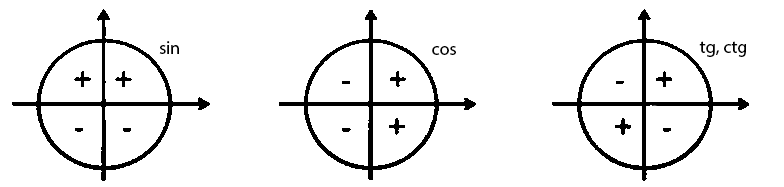
\includegraphics[scale=0.4]{1}
            
            \item \textbf{Графики}
            
            \begin{center}
                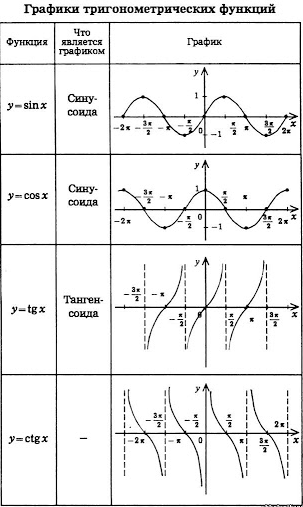
\includegraphics[scale=0.9]{2}
            \end{center}
            
        \end{enumerate}
        
        \subsection{Формулы приведения}
        
        Основные формулы:
        
        \(\sin{(t \pm \pi)} = -\sin{t}\)
        
        \(\cos{(t \pm \pi)} = -\cos{t}\)
        
        \(\sin{(\frac{\pi}{2} - t)} = \cos{t}\)
        
        \(\cos{(\frac{\pi}{2} - t)} = \sin{t}\)
        
        \begin{center}
            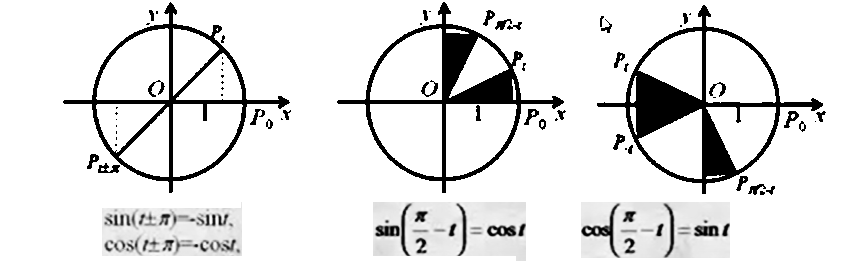
\includegraphics[scale=0.42]{3}
        \end{center}

        Другие формулы:
        
        \(\sin{(\frac{\pi}{2} + t)} = \sin{(\frac{\pi}{2} - (-t))} = \cos{(-t)} = \cos{t}\)
        
        \(\cos{(\frac{3 \pi}{2} + t)} = \cos{(2 \pi - \frac{\pi}{2} + t)} = \cos{(-\frac{\pi}{2} + t)} = \cos{(\frac{\pi}{2} - t)} = \sin{t}\)
        
        \subsection{Формулы сложения для тригонометрических функций и их следствия (формулы двойного угла, тройного угла, половинного угла)}
        
        \textbf{Определение 1.} Скалярным произведением векторов называется произведение их модулей (длин) на косинус угла между ними.
        \[\overrightarrow{a}*\overrightarrow{b} = \abs{a}\abs{b}\cos{\phi}\]
        \textbf{Замечание:} угол между векторами \(\phi\): \(0 \leq \phi \leq \pi\)
        
        \textbf{Определение 2.} Если векторы заданы своими координатами \(\overrightarrow{a} = (a_1, a_2),\ \overrightarrow{b} = (b_1, b_2)\) в ортономированном базисе (системе координат), то
        \[\overrightarrow{a}*\overrightarrow{b} = a_1 b_1 + a_2 b_2\]
        Начнём с формулы косинуса разности: \(\cos{(\alpha - \beta)}\)
        
        Итак, пусть даны числа \(\alpha\) и \(\beta\). Рассмотрим на тригонометрическом круге точки A и B, соответствующие \(\alpha\) и \(\beta\).
        
        \(\overrightarrow{OA} = \overrightarrow{a} = (\cos{\alpha}, \sin{\alpha})\) 
        \\\(\overrightarrow{OB} = \overrightarrow{b} = (\cos{\beta}, \sin{\beta})\)
        
        \(\overrightarrow{a}*\overrightarrow{b} = \cos{\alpha}\cos{\beta} + \sin{\alpha}\sin{\beta}\)
        
        С другой стороны:
        \\ \(\abs{\overrightarrow{OA}} = \abs{\overrightarrow{OB}} = 1\)
        \\а угол между ними равен "\(\beta - \alpha\)"
        \\точнее! \(\abs{\beta - \alpha} + 2 \pi k\)
        
        Так или иначе \(\cos{(\overrightarrow{OA}, \overrightarrow{OB})} = \cos{(\alpha - \beta)}\) (свойства четности и периодичности косинуса)
        
        \(\overrightarrow{a} * \overrightarrow{b} = \abs{a} \abs{b} \cos{\phi} = 1*1*\cos{(\alpha - \beta)}\)
        
        \textbf{\[\cos{(\alpha - \beta)} = \cos{\alpha}\cos{\beta} + \sin{\alpha}\sin{\beta}\]}
        
        \(\cos{(\alpha + \beta)} = \cos{(\alpha - (-\beta))} = \cos{\alpha}\cos{(-\beta)} + \sin{\alpha}\sin{(-\beta)} = \cos{\alpha}\cos{\beta} - \sin{\alpha}\sin{\beta}\)
        
        \textbf{\[\cos{(\alpha + \beta)} = \cos{\alpha}\cos{\beta} - \sin{\alpha}\sin{\beta}\]}
        
        \(\sin{(\alpha + \beta)} = \cos{(\frac{\pi}{2} - (\alpha + \beta))} = \cos{((\frac{\pi}{2} - \alpha) - \beta)} = \cos{(\frac{\pi}{2} - \alpha)}\cos{\beta} + \sin{(\frac{\pi}{2} - \alpha)}\sin{\beta} = \sin{\alpha}\cos{\beta} + \cos{\alpha}\sin{\beta}\)
        
        \textbf{\[\sin{(\alpha + \beta)} = \sin{\alpha}\cos{\beta} + \cos{\alpha}\sin{\beta}\]}
        
        \(\sin{(\alpha - \beta)} = \sin{(\alpha + (-\beta))} = \sin{\alpha}\cos{(-\beta)} + \cos{\alpha}\sin{(-\beta)} = \sin{\alpha}\cos{\beta} - \cos{\alpha}\sin{\beta}\)
        
        \textbf{\[\sin{(\alpha - \beta)} = \sin{\alpha}\cos{\beta} - \cos{\alpha}\sin{\beta}\]}
        
        \(\tg{(\alpha + \beta)} = \frac{\sin{(\alpha + \beta)}}{\cos{(\alpha + \beta)}} = \frac{\sin{\alpha}\cos{\beta} + \cos{\alpha}\sin{\beta}}{\cos{\alpha}\cos{\beta} - \sin{\alpha}\sin{\beta}} = \{\cos{\alpha}\cos{\beta} \not = 0\} = \frac{\tg{\alpha} + \tg{\beta}}{1 - \tg{\alpha}\tg{\beta}}\)
        
        О.О. левой части формулы:
        
        \(\cos{(\alpha + \beta)} \not = 0 \Leftrightarrow \alpha + \beta \not = \frac{\pi}{2} + \pi k,\ k \in \mathbb{Z}\)
        
        О.О. правой части формулы:
        
        \begin{equation}
            \begin{cases}
                \cos{\alpha} \not = 0,\\
                \cos{\beta} \not = 0,\\
                \tg{\alpha}*\tg{\beta} \not = 1
            \end{cases}\Leftrightarrow
            \begin{cases}
                \alpha \not = \frac{\pi}{2} + \pi l,\ l \in \mathbb{Z};\\
                \beta \not = \frac{\pi}{2} + \pi m,\ m \in \mathbb{Z};\\
                \cos{(\alpha + \beta)} \not = 0,\ \alpha + \beta \not = \frac{\pi}{2} + \pi n,\ n \in \mathbb{Z}.
            \end{cases}
        \end{equation}
        
        Аналогично можно получить формулы:
        
        \(\tg{(\alpha - \beta)} = \frac{\tg{\alpha} - \tg{\beta}}{1 + \tg{\alpha}\tg{\beta}}\), \(\ctg{(\alpha + \beta)} = \frac{1 - \tg{\alpha}\tg{\beta}}{\tg{\alpha} + \tg{\beta}}\), если \(\cos{\alpha} \not = 0\) и \(\cos{\beta} \not = 0\)
        
        \(\ctg{(\alpha + \beta)} = \frac{\ctg{\alpha}\ctg{\beta} - 1}{\ctg{\alpha} + \ctg{\beta}}\), если \(\sin{\alpha} \not = 0\) и \(\sin{\beta} \not = 0\) и т.д.
        
        \textbf{Следствия}
        
        \begin{enumerate}
        	\item \textbf{Формулы двойного аргумента}
            
            \(\sin{(\alpha + \beta)} = \sin{\alpha}\cos{\beta} + \cos{\alpha}\sin{\beta} \Rightarrow \sin{2\alpha} = 2\sin{\alpha}\cos{\alpha}\)
            
            \(\cos{(\alpha + \beta)} = \cos{\alpha}\cos{\beta} - \sin{\alpha}\sin{\beta} \Rightarrow \cos{2\alpha} = \cos^2{\alpha} - \sin^2{\alpha} = 1 - 2\sin^2{\alpha} = 2\cos^2{\alpha} - 1\)
            
            \(\tg{2\alpha} = \frac{2\tg{\alpha}}{1 - \tg^2{\alpha}}\)
            
            О.О. левой части снова не совпадает с О.О. правой части формулы.
            
            О.О. левой части:
            
            \(\cos{2\alpha} \not = 0 \Leftrightarrow 2\alpha \not = \frac{\pi}{2} + \pi k,\ k \in \mathbb{Z} \Leftrightarrow \alpha \not = \frac{\pi}{4} + \frac{\pi k}{2},\ k \in \mathbb{Z}\)
            
            О.О. правой части:
            
            \begin{equation}
                \begin{cases}
                    \cos{\alpha} \not = 0,\\
                    \tg^2{\alpha} \not = 1
                \end{cases}\Leftrightarrow
                \begin{cases}
                    \alpha \not = \frac{\pi}{2} + \pi l,\ l \in \mathbb{Z},\\
                    \tg{\alpha} \not = \pm 1
                \end{cases}\Leftrightarrow
                \begin{cases}
                    \alpha \not = \frac{\pi}{2} + \pi l,\ l \in \mathbb{Z},\\
                    \alpha \not = \pm \frac{\pi}{4} + \pi m,\ m \in \mathbb{Z}.
                \end{cases}
            \end{equation}
            
            \(\ctg{2\alpha} = \frac{\ctg^2{\alpha} - 1}{2\ctg{\alpha}}\)
            \\Замечание относительно О.О. в силе!
            
            Синус и косинус двойного угла можно выразить через тангенс:
            
            \(\sin{2\alpha} = \frac{2\sin{\alpha}\cos{\alpha}}{1} = \frac{2\sin{\alpha}\cos{\alpha}}{\sin^2{\alpha} + \cos^2{\alpha}} = \frac{2\tg{\alpha}}{\tg^2{\alpha} + 1}\), если \(\cos{\alpha} \not = 0\)
             
            \(\cos{2\alpha} = \frac{\cos^2{\alpha} - \sin^2{\alpha}}{1} = \frac{\cos^2{\alpha} - \sin^2{\alpha}}{\sin^2{\alpha} + \cos^2{\alpha}} = \frac{1 - \tg^2{\alpha}}{\tg^2{\alpha} + 1}\), если \(\cos{\alpha} \not = 0\)
            
            \item \textbf{Формулы тройного аргумента}
            
            \(\sin{3\alpha} = \sin{(\alpha + 2\alpha)} = \sin{\alpha}\cos{2\alpha} + \cos{\alpha}\sin{2\alpha} = \sin{\alpha}(1 - 2\sin^2{\alpha}) + 2\sin{\alpha}\cos^2{\alpha} = \sin{\alpha} - 2\sin^3{\alpha} + 2\sin{\alpha}(1 - \sin^2{\alpha}) = 3\sin{\alpha} - 4\sin^3{\alpha}\)
            
            \(\cos{3\alpha} = 4\cos^2{\alpha} - 3\cos{\alpha}\)
            
            \item \textbf{Формулы половинного угла}
            
            \(\cos{2\alpha} = 1 - 2\sin^2{\alpha} \Leftrightarrow \sin^2{\alpha} = \frac{1 - \cos{2\alpha}}{2}\)
            
            \(\cos{2\alpha} = 2\cos^2{\alpha} - 1 \Leftrightarrow \cos^2{\alpha} = \frac{1 + \cos{2\alpha}}{2}\)
            
            \(\abs{\sin{\alpha}} = \sqrt{\frac{1 - \cos{2\alpha}}{2}}\), \(\abs{\cos{\alpha}} = \sqrt{\frac{1 + \cos{2\alpha}}{2}}\) 
            
            \(\abs{\sin{\frac{x}{2}}} = \sqrt{\frac{1 - \cos{x}}{2}}\), \(\abs{\cos{\frac{x}{2}}} = \sqrt{\frac{1 + \cos{x}}{2}}\)
            
            Знак раскрытия модуля зависит от того, в какой четверти на тригонометрической окружности находится точка, соответствующая \(\frac{x}{2}\)
            
            Для тангенса и котангенса половинного аргумента можем получить:
            
            \(\abs{\tg{\frac{x}{2}}} = \sqrt{\frac{1 - \cos{x}}{1 + \cos{x}}}\)
            
            \(\abs{\ctg{\frac{x}{2}}} = \sqrt{\frac{1 + \cos{x}}{1 - \cos{x}}}\)
            
            Можно получить и другие формулы, например:
            
            \(\tg{\frac{x}{2}} = \frac{\sin{(\frac{x}{2})}}{\cos{(\frac{x}{2})}} = \frac{2\sin{(\frac{x}{2})}\cos{(\frac{x}{2})}}{2\cos^2{(\frac{x}{2})}} = \frac{\sin{x}}{1 + \cos{x}}\)
        \end{enumerate}
         
        \subsection{Произведение тригонометрических функций}
        
        Имеем:
        
        \(\cos{(\alpha - \beta)} = \cos{\alpha}\cos{\beta} + \sin{\alpha}\sin{\beta}\)
        
        \(\cos{(\alpha + \beta)} = \cos{\alpha}\cos{\beta} - \sin{\alpha}\sin{\beta}\)
        
        Путём сложения и вычитания выражений получим:
        
        \(\cos{\alpha}\cos{\beta} = \frac{1}{2}(\cos{(\alpha + \beta)} + \cos{(\alpha - \beta)})\)
        
        \(\sin{\alpha}\sin{\beta} = \frac{1}{2}(\cos{(\alpha - \beta)} - \cos{(\alpha + \beta)})\)
        
        Имеем:
        
        \(\sin{(\alpha + \beta)} = \sin{\alpha}\cos{\beta} + \cos{\alpha}\sin{\beta}\)
        
        \(\sin{(\alpha - \beta)} = \sin{\alpha}\cos{\beta} - \cos{\alpha}\sin{\beta}\)
        
        Путём сложения выражений получим:
        
        \(\sin{\alpha}\cos{\beta} = \frac{1}{2}(\sin{(\alpha + \beta)} + \sin{(\alpha - \beta)})\)
        
        \textbf{Замечание.} \(\sin^2{\alpha} = \frac{1 - \cos{2\alpha}}{2}\)
        
        \(\sin^2{\alpha} = \frac{1}{2}(\cos{0} - \cos{2\alpha}) = \frac{1 - \cos{2\alpha}}{2}\)
        
        \subsection{Сумма тригонометрических функций}
        
        \(\cos{\alpha}\cos{\beta} = \frac{1}{2}(\cos{(\alpha + \beta)} + \cos{(\alpha - \beta)})\)
        
        \(\sin{\alpha}\sin{\beta} = \frac{1}{2}(\cos{(\alpha - \beta)} - \cos{(\alpha + \beta)})\)
        
        \(\sin{\alpha}\cos{\beta} = \frac{1}{2}(\sin{(\alpha + \beta)} + \sin{(\alpha - \beta)})\)
        
        Пусть \begin{equation}
    			\begin{cases}
      				\alpha + \beta = x,\\
      				\alpha - \beta = y.
    			\end{cases}\Rightarrow
    			\begin{cases}
      				\alpha = \frac{x + y}{2},\\
      				\beta = \frac{x - y}{2}.
    			\end{cases}
			\end{equation}
        
        \(\cos x + \cos y = 2 \cos{\frac{x + y}{2}} \cos{\frac{x - y}{2}}\),
        
        \(\cos y - \cos x = 2 \sin{\frac{x + y}{2}} \sin{\frac{x - y}{2}} = -2 \sin{\frac{y - x}{2}} \sin{\frac{x + y}{2}}\),
        
        \(\sin x + \sin y = 2 \sin{\frac{x + y}{2}} \cos{\frac{x - y}{2}}\),
        
        \(\sin x - \sin y = \sin x + \sin{(-y)} = 2 \sin{\frac{x - y}{2}} \cos{\frac{x + y}{2}}\)
        
        \(\tg x \pm \tg y = \frac{\sin x}{\cos x} \pm \frac{\sin y}{\cos y} = \frac{\sin x \cos y \pm \cos x \sin y}{\cos x \cos y} = \frac{\sin{(x \pm y)}}{\cos x \cos y}\)
        
        \subsection{Введение дополнительного угла}
        
        Получим формулу для преобразования выражения \(s = a \sin x + b \cos x, a, b \not = 0\).
        
        \(s = a \sin x + b \cos x = \sqrt{a^2 + b^2}(\frac{a}{\sqrt{a^2 + b^2}} \sin x + \frac{b}{\sqrt{a^2 + b^2}} \cos x)\)
        
        Заметим, что \(\abs{\frac{a}{\sqrt{a^2 + b^2}}} \leq 1,\ \abs{\frac{b}{\sqrt{a^2 + b^2}}} \leq 1\) и \((\frac{a}{\sqrt{a^2 + b^2}})^2 + (\frac{b}{\sqrt{a^2 + b^2}})^2 = 1 \Rightarrow\ \exists\ \phi\).
        
        \(\sin{\phi} = \frac{a}{\sqrt{a^2 + b^2}},\ \cos{\phi} = \frac{b}{\sqrt{a^2 + b^2}}\) или \(\exists\ \psi : \cos{\psi} = \frac{a}{\sqrt{a^2 + b^2}},\ \sin{\psi} = \frac{b}{\sqrt{a^2 + b^2}}\).
        
        Тогда \begin{enumerate}
        	\item \(s = \sqrt{a^2 + b^2}(\sin{\phi} \sin x + \cos{\phi} \cos x) = \sqrt{a^2 + b^2} \cos{(x - \phi)}\) или
            \item \(s = \sqrt{a^2 + b^2}(\cos{\psi} \sin x + \sin{\psi} \cos x) = \sqrt{a^2 + b^2} \sin{(x + \psi)}\).
        \end{enumerate}
        
        \subsection{Обратные тригонометрические функции, их основные свойства (ОО, ОЗ, графики, чётность, монотонность)}
        
        \subsubsection{Арксинус}
        
        \textbf{Определение.} Функция, обратная к функции \(y = \sin x\), рассмотренной на промежутке \([-\frac{\pi}{2}; \frac{\pi}{2}]\), называется арксинусом и обозначается \(x = \arcsin y\), где y --- аргумент, а x --- значение функции
    	
        \textbf{О.О.} \(x \in [-1; 1]\)(из определения)
        
        \textbf{О.З.} \(y \in [-\frac{\pi}{2}; \frac{\pi}{2}]\)(из определения)
        
        \textbf{Графики}
        \begin{center}
            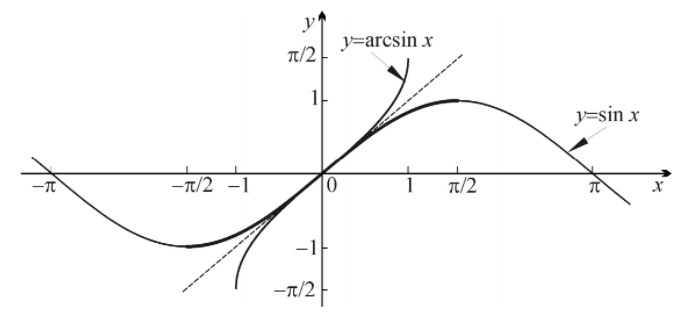
\includegraphics[scale=0.4]{4}
        \end{center}
        
        \textbf{Чётность.} Арксинус --- нечётная функция: \(\arcsin{(-x)} = -\arcsin x\)
        
        \(\uparrow\) Обозначим \(\phi = \arcsin{(-x)}\) --- такое число, что по определению арксинуса \(-\frac{\pi}{2} \leq -\phi \leq \frac{\pi}{2}\) и \(\sin{\phi} = -x\). Но тогда, в силу свойств неравенств и нечетности синуса, получаем
        \(-\frac{\pi}{2} \leq -\phi \leq \frac{\pi}{2}\) и \(\sin{(-\phi)} = x\). Эти выражения по определению арксинуса означают, что \(-\phi = \arcsin x\).
        Из последнего равенства следует, что \(\phi = -\arcsin x\) или, возвращаясь к исходным обозначениям, \(\arcsin{(-x)} = -\arcsin x\ \downarrow\)
        
        \textbf{Монотонность.} Арксинус есть функция непрерывная и возрастающая на области определения
        
        \subsubsection{Арккосинус}
        
        \textbf{Определение.} Функция, обратная к функции \(y = \cos x\), рассмотренной на промежутке \([0; \pi]\), называется арккосинусом и обозначается \(x = \arccos y\), где y --- аргумент, а x --- значение функции
        
        \textbf{О.О.} \(x \in [-1; 1]\)(из определения)
        
        \textbf{О.З.} \(y \in [0; \pi]\)(из определения)
        
        \textbf{Графики}
        \begin{center}
            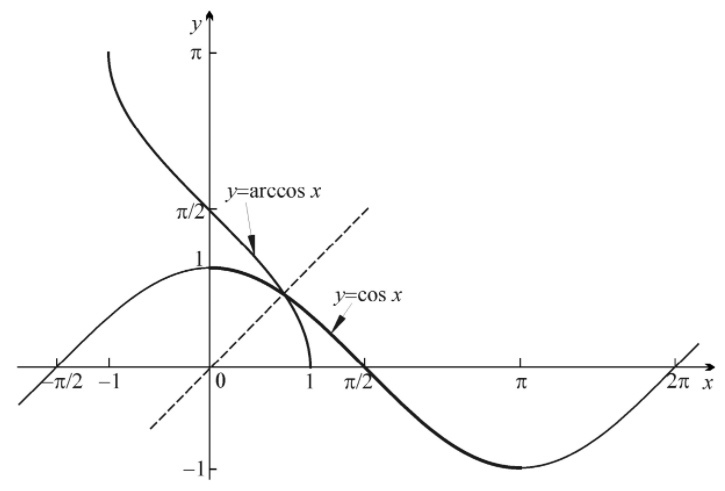
\includegraphics[scale=0.4]{5}
        \end{center}
        
        \textbf{Чётность.} Арккосинус --- ни чётная, ни нечётная функция: \(\arccos{(-x)} = \pi - \arccos x\)
        
        \(\uparrow\) Обозначим \(\phi = \arccos{(-x)}\) --- такое число, что по определению арккосинуса \(0 \leq \phi \leq \pi\) и \(\cos{\phi} = -x\). Но тогда, в силу свойств неравенств и формул приведения, получаем
        \(0 \leq \pi-\phi \leq \pi\) и \(x = \cos{(\pi - \phi)}\). Эти выражения по определению арккосинуса означают, что \(\pi-\phi = \arccos x\).
        Из последнего равенства получаем, что \(\phi = \pi-\arccos x\) или, возвращаясь к исходным обозначениям, \(\arccos{(-x)} = \pi - \arccos x \ \downarrow\)
        
        \textbf{Монотонность.} Арккосинус есть функция непрерывная на промежутке \([-1; 1]\) и монотонно убывает на нём от \(\pi\) до 0
        
        \subsubsection{Арктангенс}
        
        \textbf{Определение.} Функция, обратная к функции \(y = \tg x\), рассмотренной на промежутке \((-\frac{\pi}{2}; \frac{\pi}{2})\), называется арктангенсом и обозначается \(x = \arctg y\), где y --- аргумент, а x --- значение функции
        
        \textbf{О.О.} \(x \in (-\infty; +\infty)\)(из определения)
        
        \textbf{О.З.} \(y \in (-\frac{\pi}{2}; \frac{\pi}{2})\)(из определения)
        
        \textbf{Графики}
        \begin{center}
            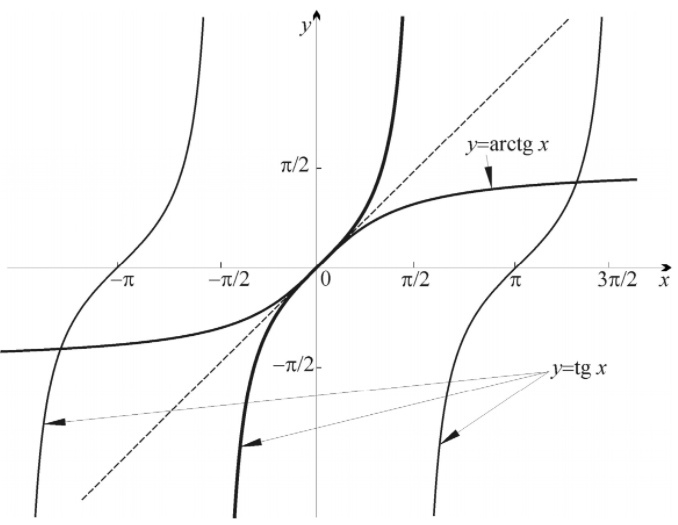
\includegraphics[scale=0.4]{6}
        \end{center}
        
        \textbf{Чётность.} Арктангенс --- нечётная функция: \(\arctg{(-x)} = -\arctg x\)
        
        \(\uparrow\) Обозначим \(\phi = \arctg{(-x)}\) --- такое число, что по определению арктангенса \(-\frac{\pi}{2} < -\phi < \frac{\pi}{2}\) и \(\tg{\phi} = -x\). Но тогда, в силу свойств неравенств и нечетности тангенса, получаем
        \(-\frac{\pi}{2} < -\phi < \frac{\pi}{2}\) и \(\tg{(-\phi)} = x\). Эти выражения по определению арктангенса означают, что \(-\phi = \arctg x\).
        Из последнего равенства следует, что \(\phi = -\arctg x\) или, возвращаясь к исходным обозначениям, \(\arctg{(-x)} = -\arctg x\ \downarrow\)
        
        \textbf{Монотонность.} Арктангенс есть функция непрерывная на всей числовой оси и монотонно возрастающая на ней от \(-\frac{\pi}{2}\) до \(\frac{\pi}{2}\)
        
        \subsubsection{Арккотангенс}
        
        \textbf{Определение.} Функция, обратная к функции \(y = \ctg x\), рассмотренной на промежутке \((0; \pi)\), называется арккотангенсом и обозначается \(x = \arcctg y\), где y --- аргумент, а x --- значение функции
        
        \textbf{О.О.} \(x \in (-\infty; +\infty)\)(из определения)
        
        \textbf{О.З.} \(y \in (0; \pi)\)(из определения)
        
        \textbf{Графики}
        \begin{center}
            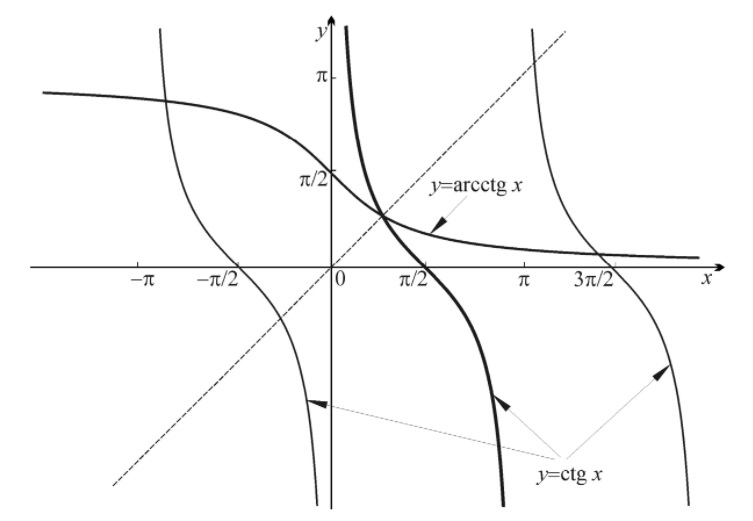
\includegraphics[scale=0.4]{7}
        \end{center}
        
        \textbf{Чётность.} Арккотангенс --- ни чётная, ни нечётная функция: \(\arcctg{(-x)} = \pi - \arcctg x\)
        
        \(\uparrow\) Обозначим \(\phi = \arcctg{(-x)}\) --- такое число, что по определению арккотангенса \(0 < \phi < \pi\) и \(\ctg{\phi} = -x\). Но тогда, в силу свойств неравенств и формул приведения, получаем
        \(0 < \pi-\phi < \pi\) и \(x = \ctg{(\pi - \phi)}\). Эти выражения по определению арккотангенса означают, что \(\pi-\phi = \arcctg x\).
        Из последнего равенства получаем, что \(\phi = \pi-\arcctg x\) или, возвращаясь к исходным обозначениям, \(\arcctg{(-x)} = \pi - \arcctg x \ \downarrow\)
        
        \textbf{Монотонность.} Арккотангенс есть функция непрерывная на всей числовой оси и монотонно убывающая на ней от \(0\) до \(\pi\)
    
    \section{Действительные числа}
        \subsection{Введение. Задача измерения отрезков}
            $a_{\in \mathbb{N}} + x = b_{\in \mathbb{N}}$ есть алгебраическая предпосылка для возникновения целых чисел.
            
            $\mathbb{Z} = \mathbb{N}^{+} \cup \mathbb{N}^{-} \cup \{0\}$
            
            Свойства для $\mathbb{N}$ сохраняем в $\mathbb{Z}$:

            \begin{enumerate}
                \item $a + b = b + a$
                \item $a + (b + c) = (a + b) + c$
                \item $ab = ba$
                \item $a(bc) = (ab)c$
                \item $a(b + c) = ab + ac$
            \end{enumerate}
            
            $a_{\in \mathbb{Z} \textrm{\textbackslash} \{0\}}x = b_{\in \mathbb{Z}}$ есть алгебраическая предпосылка для возникновения рациональных чисел $\mathbb{Q}$
            
            O------------------------A\\
            O-----E
            
            $OE$ --- единичный отрезок

            $\abs{OA} = n \abs{OE}$
            
            \textbf{Определение.} Отрезки $a$ и $b$ называются соизмеримыми, если $\exists$ отрезок $c$:
            
            $\abs{a}=n\abs{c}$\\
            $\abs{b}=m\abs{c}$, $m,\ n \in \mathbb{N}$

            $\abs{a} = \frac{n}{m}\abs{b}$
            
            \textbf{Определение.} Числа вида $\frac{n}{m}$, где $m \in \mathbb{N},\ n \in \mathbb{Z}$ назовем рациональными.

            \underline{Между любыми двумя рациональными числами $\exists\ \infty$ число других рациональных чисел}

            Например, между $r_1$ и $r_2$ существует $\frac{r_1 + r_2}{2}$ и т.д.

            \underline{Множество $\mathbb{Q}$ --- ``всюду плотно``} 

            \underline{Существуют несоизмеримые отрезки:}

            Нарисуем квадрат со стороной $x$ и диагональю $y$.
            $x^2$ + $x^2$ = $y^2$.
            Если они соизмеримы, то $y = rx$.
            $\not\exists\ r \in \mathbb{Q}: r^2 = 2$

            От противного:

            Пусть $\exists\ r = \frac{n}{m}$ --- несократимая $\Rightarrow \frac{n^2}{m^2} = 2 \Rightarrow n^2 = 2m^2 \Rightarrow n = 2k \Rightarrow 4k^2 = 2m^2 \Rightarrow 2k^2 = m^2 \Rightarrow m^2 \vdots 2 \Rightarrow m \vdots 2 \Rightarrow$ дробь сократима --- противоречие.

            \underline{Это возникновение иррациональных чисел}

        \subsection{Бесконечные десятичные дроби}
            Будем рассматривать десятичные дроби:
            \begin{enumerate}
                \item конечная десятичная дробь.\\
                $\abs{OA} = 4,806 = 4_{= 4\ \abs{OE}_{= e}} + \frac{8}{10} + \frac{6}{1000}$\\
                \item $\abs{OA} = \frac{1}{3}?$\\
                $\frac{1}{3} = \frac{m}{10^n} \quad 10^n = 3m$ невозможно\\
                Но можно измерять со все больше возрастающей точностью\\
                $|_{0}----|----|_{N}----|_{N+1}---->$\\
                $O-----------A$\\
                \begin{enumerate}[1.]
                    \item Делим $OX$ на отрезки равные 1, т.е. рассмотрим $[n; n+1] \Rightarrow$ пусть $A$ попала в $[N; N+1]$
                    \item $|_{N}--|--|_{A}--|--|_{N}--|_{N+1}$\\
                    $[N,m_1;N,m_1 + \frac{1}{10}]$\\
                    $[N,n_1;N,n_1 + \frac{1}{10}]$ --- это тот куда попал $A$\\
                    $[N,n_1n_2;N,n_1n_2 + \frac{1}{100}]$ и т.д.\\
                \end{enumerate}
            \end{enumerate}

        $[N; N+1] = I_0$\\
        $[N,n_1; N,n_1 + \frac{1}{10}] = I_1$\\
        $[N,n_1n_2; N,n_1n_2 + \frac{1}{100}] = I_2$\\
        $...$\\
        $[N,n_1n_2...n_k; N,n_1n_2...n_k + \frac{1}{10^k}] = I_k$\\
        $...$\\
        Это процесс(*)!!!

        $I_0 \supset I_1 \supset I_2 \supset ... \supset I_k \supset ...$

        $\alpha_k = N,n_1n_2...n_k \quad \nearrow$

        $\alpha_k' = N,n_1n_2...n_k + \frac{1}{10^k} \quad \searrow$ 

        \textbf{Определение.} Этот процесс (*) принято называть бесконечной десятичной дробью и обозначается\\ 
        $\alpha = N,n_1n_2...n_k...$
        
        \textbf{Определение.} Число $\alpha_k = N,n_1n_2...n_k$ --- приближение $\alpha$ по недостатку с точностю до $\frac{1}{10^k}$

        \textbf{Определение.} Число $\alpha_k' = N,n_1n_2...n_k + \frac{1}{10^k}$ --- приближение $\alpha$ по избытку с точностю до $\frac{1}{10^k}$

        В общем случае процесс (*), кроме случая конечной десятичной дроби.

        Например:
        \[0,45\]
        \[[0,4; 0,5]\]
        \[\textrm{процесс раздвоился}\]
        \[[0,44; 0,45]\quad|\quad[0,45; 0,46]\]
        \[[0,449; 0,450]\quad|\quad[0,450; 0,451]\]
        \[[0,4499; 0,4500]\quad|\quad[0,4500; 0,4501]\]
        \[...\]
        \[\cancel{0,44999...(9)} \textrm{(такие числа не рассматриваем)}\quad\quad 0,4500000...(0)\]

        \textbf{Определение.} Положительным действительным числом называем всякую бесконечную десятичную\\ дробь, не оканчивающуюся последовательностью 9-ок.

        \textbf{Определение.} Число $\beta$ назовем отрицательным действительным числом, если $\beta = -\alpha = -N,n_1n_2...n_k...$

        $0 = 0,000...0...$\\
        $\cancel{0 = -0,000...0...}$

        $\alpha = [\alpha_k; \alpha_k']$

        $-\alpha = \beta = [-\alpha_k'; -\alpha_k]$

        \textbf{Свойства.}

        \begin{enumerate}[0.]
            \item Действительные числа можно сравнивать
            \begin{enumerate}[1.]
                \item \[\alpha, \beta > 0;\ \alpha = N,n_1n_2...n_k...;\ \beta = M,m_1m_2...m_k...\]
                \[N < M \Rightarrow \alpha < \beta, N = M, N > M \Rightarrow \alpha > \beta\]
                \[\Downarrow\]
                \[n_1 < m_1 \Rightarrow \alpha < \beta, n_1 = m_1, n_1 > m_1 \Rightarrow \alpha > \beta\]
                \[\Downarrow\]
                \[...\]
                \item \[\alpha < 0, \beta > 0 \Rightarrow \alpha < \beta\]
                \item \[\alpha < 0, \beta < 0 \Rightarrow \alpha > \beta \Leftrightarrow -\alpha < -\beta\]
            \end{enumerate}
        \end{enumerate}

        \subsection{Рациональные числа и бесконечные десятичные дроби}
        \textbf{Утверждение.} Всякое рациональное число можно записать в виде бесконечной десятичной дроби. 

        $\frac{2}{5} = 0,4(0)...$

        $\frac{5}{11} = 0,(45)...$

        $\frac{1}{7} = 0,(142857)...$

        $\frac{8}{45} = 0,1(7)...$

        \textbf{Определение.} Период - повторяющаяся группа цифр.

        \textbf{Определение.} Длина периода - число цифр.

        \textbf{Утверждение.} Всякое рациональное число представимо в виде \underline{периодической} бесконечной десятичной дроби.

        $\uparrow$ Достаточно доказать для правильных дробей.

        $\frac{m}{n}$

        Остатки при делении на $n$?

        $0_{\textrm{с этим легко}}, 1, 2, 3, 4, ..., n - 1$

        Остался $n - 1$ остаток

        Не более чем через $n - 1$ чисел возникает второй раз остаток, который уже был. Далее остатки будут повторяться.

        \underline{Итог:} Иррациональные числа - непериодические бесконечные десятичные дроби. 

        \subsection{Разделяющее число числовых множеств}
        Некоторую совокупность действительных чисел назовем числовым множеством.
        
        Само множество действительных чисел обозначается $\mathbb{R}$.
        
        Другими примерами числовых множеств могут служить:
        
        $\mathbb{R}+$ --- множество положительных действительных чисел.
        
        $\mathbb{Q}-$ --- множество отрицательных рациональных чисел.
        
        $(-\infty; a]$ --- множество действительных чисел $x: x \leq a$.

        \textbf{Определение.} Числовое множество $X$ называется ограниченным, если $\exists\ M \in \mathbb{R}: \forall\ x \in X: \abs{x} \leq M$.

        \textbf{Определение.} Будем говорить, что множество $B$ лежит справа от множества $A$, если $\forall\ x \in A$ и $\forall\ y \in B: x \leq y \quad A, B \subset \mathbb{R}$.

        

        \textbf{Определение.} Число $c \in \mathbb{R}$ называется разделяющим числом для множества $A$ и $B \subset \mathbb{R}$, если $\forall\ a \in A$ и $\forall\ b \in B: a \leq c \leq b$.

        Из определения следует, что если для множеств $A$ и $B$ существует разделяющее число, то $B$ лежит справа от множества $A$. Верно и обратное утверждение.

        \textbf{Теорема.} Пусть $A$ и $B$ два числовых множества. Причем множество $B$ лежит справа от множества $A$.\\
        Тогда $\exists$ по крайней мере одно число $c$, разделяющее эти множества.

        $\uparrow$
        Рассмотрим единичные отрезки вида $[n,n+1]$.
            
        Для множества $B$ рассмотрим самый левый из отрезков $[n,n+1]$, содержащий элементы этого множества (если самый маленький $b$ попал на границу, то берем «достаточный отрезок»). Обозначим этот отрезок $[N,N+1]$. Для простоты будем считать, что $N \geq 0$.
        
        Для множества $A$ рассмотрим самый правый из отрезков $[n,n+1]$. Пусть это $[M,M+1]$. 

        \begin{enumerate}
            \item $M > N$ --- невозможно (так как тогда есть $a > b$);
            \item $M < N$ --- тогда в качестве разделяющего числа можно взять, например, $c = N.\quad \forall\ a \in A,\ \forall\ b \in B \quad a \leq c \leq b$.
            \item $M = N \Rightarrow$ 
        \end{enumerate}

        Разделим $[N,N+1]$ на $10$ частей $\Rightarrow [N + \frac{n_1}{10},N + \frac{n_1 + 1}{10}], n_1 = 0,1,2,...,9$.

        Снова выбираем $N_1: [N + \frac{N_1}{10},N + \frac{N_1 + 1}{10}]$ --- самый левый (с замечанием) из таких отрезков, содержащий элементы из $B$, и $M_1: [N + \frac{M_1}{10},N + \frac{M_1 + 1}{10}]$ --- самый правый из таких отрезков, содержащий элементы из $A$. 

        \begin{enumerate}
            \item $M_1 > N_1$ --- невозможно (так как тогда есть $a > b$);
            \item $M_1 < N_1$ --- тогда в качестве разделяющего числа можно взять, например, $c = N,N_1.\quad \forall\ a \in A,\ \forall\ b \in B \quad a \leq c \leq b$.
            \item $M_1 = N_1 \Rightarrow$ 
        \end{enumerate}

        Полученный $[N + \frac{N_1}{10},N + \frac{N_1 + 1}{10}] = [N,N_1; N,N1+\frac{1}{10}]$ снова делим на $10$ частей. И снова выбираем самый левый промежуток, содержащий элементы из $B$, и самый правый, содержащий элементы из $A$. И т.д.

        В итоге, мы либо найдем $c$, либо в самом «тяжелом случае» построим систему вложенных промежутков: 

        $[N,N + 1] \supset [N,N_1; N,N_1 + \frac{1}{10}] \supset [N,N_1N_2; N,N_1N_2 + \frac{1}{100}] \supset ...$

        Возьмем в качестве $c$ б.д.д., отвечающую этому процессу: $c = N,N_1N_2...N_k...$

        Это $c$ и будет разделяющим числом.
        
        Действительно, покажем, что $\forall\ b \in B\ c \leq b$.

        От противного. Если существует $b < c$, то из упорядоченности действительных чисел при большом $l$ точки $b$ и $c$ попали бы в разные отрезки длины $\frac{1}{10^l}$, и выбранный малый промежуток не был бы самым левым для множества $B. \Rightarrow c \leq b$

        Аналогично $\forall\ a \in A\ a \leq c$.

        Остались неосвещенными моменты: $c$ оканчивается последовательностью 9-ок, для $N < 0$. $\downarrow$

        \subsection{Теорема о разноцветных отрезках (единственность разделяющего числа)}
        \textbf{Определение.} Пусть множество $B$ лежит справа от $A$. Назовем отрезок $[a; b]$ разноцветным, если $a \in A, b \in B$.

        \textbf{Определение.} Будем говорить, что существует система сколь угодно малых разноцветных отрезков, если $\forall\ \varepsilon > 0$ (каким бы маленьким мы его не взяли) $\exists$ разноцветные отрезки $[a; b]$ и $[\alpha; \beta]$ ($[\alpha; \beta] \supset [a; b], \alpha, \beta$ --- рациональные числа): $\beta - \alpha < \varepsilon$. 

        \textbf{Замечание.}

        \begin{enumerate}
            \item Так как $\forall\ \varepsilon$, то таких отрезков сколь угодно много (система).
            \item Координаты $\alpha, \beta$ --- рациональные числа нужны нам, так как действия с действительными числами ещё не вводились. Мы не знаем, что есть $a - b$. Если бы знали, то просто писали бы: $\exists$ разноцветные отрезки $[a; b]: b - a < \varepsilon$.
        \end{enumerate}

        \textbf{Теорема.} Пусть множество $B$ лежит справа от $A$. Для того, чтобы $A$ и $B$ разделялись лишь одним числом необходимо и достаточно, чтобы $\exists$ система сколь угодно малых разноцветных отрезков. 

        $\uparrow$ Необходимость ``$\Leftarrow$``. Пусть существует система сколь угодно малых разноцветных отрезков, покажем, что $\exists! c$. 

        От противного. Пусть $\exists$ два разделяющих числа $c_1$ и $c_2$ (для определенности $c_1 < c_2$). При достаточно большом $n$ числа $c_1$ и $c_2$ принадлежат отрезкам деления числовой оси длины $\frac{1}{10^n}$, не имеющими общих концов (это следует из упорядоченности действительных чисел). Т.е. между $c_1$ и $c_2$ существует хотя бы один отрезок $[\frac{m}{10^n}; \frac{m + 1}{10^n}]: c_1 < \frac{m}{10^n} < \frac{m + 1}{10^n} < c_2$.
        
        Но тогда, $\forall\ a \in A, b \in B\ a \leq c_1 < c_2 \leq b$, а потому $d =\ $(длина любого отрезка с рациональными концами, содержащего $[a; b]$) $> \frac{1}{10^n}$. Противоречие с существованием системы сколь угодно малых разноцветных отрезков.

        Достаточность ``$\Rightarrow$``. Пусть $\exists! c$, покажем существование системы сколь угодно малых разноцветных отрезков.

        $c$ --- единственное разделяющее число. Зададим $\varepsilon > 0$ и возьмём $[\alpha, \beta]$ c рациональными концами такой, что $\alpha < c < \beta$. Например, если $c_n$ --- приближение $c$ по недостатку с точностью до $\frac{1}{10^n}$, то можем рассмотреть целую систему таких промежутков: $[\alpha_n; \beta_n] = [c_n - \frac{1}{10^n}; c_n + \frac{1}{10^n}]$. 

        Покажем, что на любом отрезке такого вида есть, хотя бы одно число из $A$. От противного: пусть нет, тогда $\forall\ a \in A a < \alpha_n$, при этом $\forall\ b \in B b \geq c$. Тогда все числа из $[\alpha_n; c]$ разделяют $A$ и $B$. Аналогично, можно показать, что на любом отрезке такого вида есть, хотя бы одно число из $B$. Значит любой такой $[\alpha_n; \beta_n] \supset [a_n; b_n]$ --- разноцветный.

        $\beta - \alpha = \frac{2}{10^n} < \{10^n = (1 + 9)^n > 9n\} < \frac{2}{9n} < \varepsilon_k < \varepsilon$, где $N \geq [\frac{2}{9 \varepsilon_k}] + 1. \downarrow$ 

        \textbf{Пример.} Покажем, что отрезки $[1; 4] [4; 8]$ разделяются лишь числом $4$.
        
        Заметим, что отрезки $[4 - \frac{1}{n}; 4 + \frac{1}{n}]$ --- разноцветные. Их длина $d = \frac{2}{n}$ путем выбора $n$ может быть сделана меньше любого наперед заданного действительного $\varepsilon$. Если $\frac{2}{n} < \varepsilon_k < \varepsilon$, то $n \geq [\frac{2}{\varepsilon_k}] + 1$. 

        \textbf{Пример.} Найти разделяющее число множеств $A = \{ \frac{n^2}{n^2 + 1}, n \in \mathbb{N} \}$ и $B = \{ \frac{n^2 + 2}{n^2 + 1}, n \in \mathbb{N} \}$

        Заметим, что $\frac{n^2}{n^2 + 1} = \frac{n^2 + 1 - 1}{n^2 + 1} = 1 - \frac{1}{n^2 + 1} < 1, \frac{n^2 + 2}{n^2 + 1} = \frac{n^2 + 1 + 1}{n^2 + 1} = 1 + \frac{1}{n^2 + 1} > 1$. Т.е. множество $B$ лежит справа от $A$. Докажем, что $1$ --- единственное разделяющее число этих множеств. Отрезки $[1 - \frac{1}{n^2 + 1}; 1 + \frac{1}{n^2 + 1}]$ разноцветные, их длина $d = \frac{2}{n^2 + 1} < \frac{2}{n^2} < \frac{1}{n} < \varepsilon_k < \varepsilon \Rightarrow n \geq [\frac{2}{\varepsilon_k}] + 1$.

        \subsection{Арифметические операции над действительными числами}

        \textbf{\underline{Сложение}}
        
        Пусть заданы $x, y \in \mathbb{R}$. Рассмотрим два множества:

        $A = \{p + q, \textrm{ где } p \in \mathbb{Q}, p \leq x, q \in \mathbb{Q}, q \leq y\}$, 

        $B = \{r + s, \textrm{ где } r \in \mathbb{Q}, r \geq x, s \in \mathbb{Q}, s \geq y\}$.

        Так как $p \leq x \leq r$, $q \leq y \leq s \Rightarrow p + q \leq r + s$, значит множество $B$ лежит справа от $A \Rightarrow$ существует по крайней мере одно разделяющее число для этих множеств. 

        \textbf{Утверждение.} Покажем, что разделяющее число существует единственное.

        Для этого достаточно показать существование системы сколь угодно малых разноцветных отрезков. 

        Пусть десятичное приближение по недостатку с точностью $\frac{1}{10^n}$ для $x$ --- это $\frac{l}{10^n}$, а для $y$ --- $\frac{m}{10^n}$. Тогда $\frac{l}{10^n} \leq x < \frac{l + 1}{10^n}$, $\frac{m}{10^n} \leq x < \frac{m + 1}{10^n}$. Тогда $\frac{l}{10^n} + \frac{m}{10^n} \in A$, а $\frac{l + 1}{10^n} + \frac{m + 1}{10^n} \in B$. Но $d = (\frac{l + 1}{10^n} + \frac{m + 1}{10^n}) - (\frac{l}{10^n} + \frac{m}{10^n}) = \frac{2}{10^n} < \frac{2}{9n} < \varepsilon_k < \varepsilon$. Т.е. существуют сколь угодно маленькие разноцветные отрезки. 

        Это единственное число, разделяющее множества $A$ и $B$, называют суммой $x + y$.

        \textbf{Определение.} Суммой действительных чисел $x$ и $y$ называют такое число $x + y$, которое является единственным разделяющим числом для сумм $p + q (p \leq x, q \leq y, p,q \in \mathbb{Q})$ и сумм $r+s (r \geq x, s \geq y, r,s \in \mathbb{Q})$.
        
        \textbf{\underline{Разность}}

        \textbf{Определение.} Разностью действительных чисел $x$ и $y$ назовем сумму $x$ и $(-y)$.
        
        \textbf{\underline{Умножение}}

        (I)

        $x, y > 0$

        $A = \{pq, p, q \in \mathbb{Q}^{+}: p \leq x; q \leq y\} (*)$

        $B = \{rs, r, s \in \mathbb{Q}^{+}: x \leq r; y \leq s\} (*)$

        Легко понять, что $pq \leq rs \Rightarrow B$ лежит справа от $A \Rightarrow \exists$ хотя бы одно разделяющее число $c$.

        \textbf{Утверждение.} $\exists! c$ для $A$ и $B$ (*)

        (II)

        Если $x, y$ не $> 0$, то произведение вводится в соответствии с правилом знаков. 

        $(-x)y = x(-y) = -xy$

        и 

        $(-x)(-y) = xy$

        Свойства (доказываются из свойств рациональных чисел):

        \begin{enumerate}
            \item $xy = yx$
            \item $x(yz) = (xy)z$
            \item $x(y + z) = xy + xz$
        \end{enumerate}

        Остается в силе:

        $0 * x = x * 0 = 0, \forall\ x \in \mathbb{R}$

        $1 * x = x * 1 = x, \forall\ x \in \mathbb{R}$

        \textbf{\underline{Деление}}

        $x > 0$ Поймем, что есть $\frac{1}{x}$

        $A = \{\frac{1}{p}, p \in \mathbb{Q}^{+}: p \geq x\}$ (**)

        $B = \{\frac{1}{q}, q \in \mathbb{Q}^{+}: q \leq x\}$ (**)

        $q \leq p \in \mathbb{Q}^{+} \Rightarrow \frac{1}{p} \leq \frac{1}{q} \Rightarrow$ множество $B$ лежит справа от $A$.
        
        $\Downarrow$

        $\exists$ хотя бы одно разделюящее число.

        \textbf{Утверждение.} $\exists! c$ для $A$ и $B$ (**)

        Если $x = 0: \not\exists\ \frac{1}{x}$
        
        Если $x < 0: \frac{1}{x} = -\frac{1}{-x}$

        $x, y \in \mathbb{R}:\quad y \neq 0 \quad \frac{x}{y} = x*(\frac{1}{y})$

        Свойство:

        $x*\frac{1}{x} = 1 \quad \forall x \neq 0$

        Множество $\mathbb{R}$ замкнуто относительно четырех арифметических операций.

        $\mathbb{R}$ --- числовое поле.

        \subsection{Превращение бесконечных периодических десятичных дробей в обыкновенные}

        \textbf{Пример.}
        
        $0,(54)$

        $x = 0,(54)$

        $100x = 54,(54)$

        $99x = 54$

        $x = \frac{54}{99} = \frac{6}{11}$

        \textbf{Пример.}

        $0,(351)$

        $x = 0,(351)$

        $1000x = 351,(351)$

        $999x = 351$

        $x = \frac{351}{999}$

        \textbf{Пример.}

        $0,47(612)$

        $x = 0,47(612)$

        $x * 10^5 = 47612,(612)$

        $x * 10^2 = 47,(612)$

        $x = \frac{47612 - 47}{10^2 * 999}$

        \subsection{Рациональное и иррациональное число. Плотность этих множеств в R}
        \textbf{Утверждение.} Для $\forall\ x, y \in \mathbb{R} \exists$ отрезок с рациональными концами: он лежит между $x$ и $y$. (***)

        $\uparrow$

        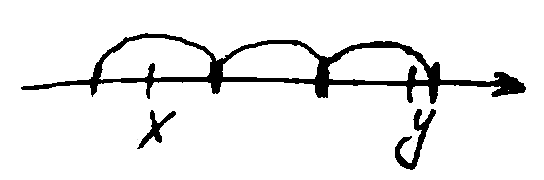
\includegraphics[scale=0.2]{d_ch_8}

        $x, y \in \mathbb{R}, x < y$

        $\exists$ разбиение отрезками длины $\frac{1}{10^n}$, что $x$ и $y$ лежат в отрезках такой длины и не имещих общих концов: это отрезки вида $[\frac{m}{10^n}_{ = r \in \mathbb{Q}}; \frac{m + 1}{10^n}] = [r, r + \frac{1}{10^n}] \downarrow$
        
        \textbf{Утверждение.} Между любыми $x, y \in \mathbb{R}, x \subset y \exists\ \infty$ число рациональных чисел.

        $\uparrow$

        Уже в утверждении (***) показали, что $\exists$ между $x$ и $y$ $[r_{\in \mathbb{Q}}, r + \frac{1}{10^n}_{\in \mathbb{Q}}] = [r_1, r_2] \Rightarrow r_1 < \frac{r_1 + r_2 = r_3}{2} < r_2$

        $r_1 < \frac{r_1 + r_3}{2} < r_3 < \frac{r_3 + r_2}{2} < r_2$ и т.д. $\downarrow$

        \textbf{Утверждение.} Между $x$ и $y \in \mathbb{R} x < y \exists\ \infty$ число иррациональных чисел.

        $\uparrow$

        Покажем, что между любыми двумя рациональными числами $\exists$ хотя бы одно иррациональное.

        Уже между $x$ и $y \exists\ [r, r + \frac{1}{10^m}] = [r_1, r_2]$ 

        $r_1 = \alpha,\alpha_1\alpha_2...\alpha_m \quad r_2 = r_1 + \frac{1}{10^m}$

        Легко понять, что $\beta = \alpha,\alpha_1...\alpha_m00100111$ (допишем заведомо непериодический конец) $\downarrow$

        \textbf{Определение.} Числовое множество $A$ эквивалентно множеству $B$, если $\exists$ взаимнооднозначное отображение $A$ в $B$.

        \textbf{Определение.} Числовое множество $A$ называется счетным, если оно эквивалентно множеству $\mathbb{N}$. (т.е. все элементы $A$ можно пронумеровать).

        \textbf{Утверждение.} Множество рациональных чисел счётно. 

        $\uparrow$

        \underline{Способ 1} $\frac{p}{q}$ --- рациональное, если $p \in \mathbb{Z}, q \in \mathbb{N}$

        $s = \abs{p} + q$ --- высота рационального числа.

        $s = 1 \quad \frac{0}{1} \quad 1 $ист

        $s = 2 \quad \frac{1}{1} - \frac{1}{1} \cancel{\frac{0}{2}} \quad 3$ ист

        $s = 3 \quad \frac{\pm 2}{1} \frac{\pm 1}{2} \cancel{\frac{0}{3}} \quad 5$ ист

        $s:$ не более $2(s - 1) + 1 = 2s - 1$ ист --- конечное число и т.д. все занумерую.

        \underline{Способ 2} 
        --- - линия, вдоль которой нумерую, вычеркивая повторяющиеся.

        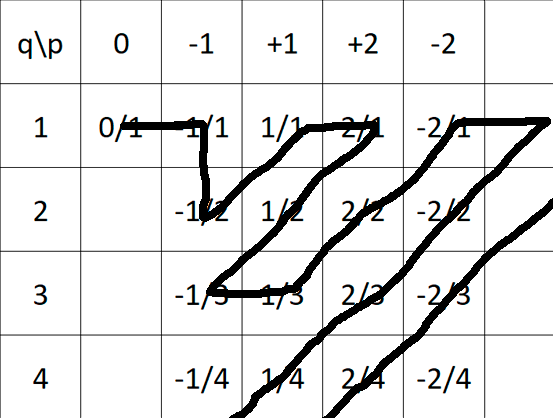
\includegraphics[scale=0.4]{d_ch_8_1}

        $\downarrow$

        \textbf{Утверждение.} Множество $\mathbb{R}$ --- несчетное множество.

        $\uparrow$

        Остается полагать, что (0; 1) --- несчетное множество.

        От противного. Пусть счетное, тогда нумерую все элементы.

        Обозначим эту группу (****)

        $r_1 = 0,a_{11}a_{12}a_{13}...a_{1n}...$

        $r_2 = 0,a_{21}a_{22}a_{23}...a_{2n}...$

        $r_3 = 0,a_{31}a_{32}a_{33}...a_{3n}...$

        $r_n = 0,a_{n1}a_{n2}a_{n3}...a_{nn}...$

        и т.д.

        $\beta = 0,\beta_1\beta_2...\beta_n...$

        $\beta_1 \neq a_{11} \neq 9 \Rightarrow \beta \neq r_1$
        
        $\beta_2 \neq a_{22} \neq 9 \Rightarrow \beta \neq r_2$
        
        $\beta_3 \neq a_{33} \neq 9 \Rightarrow \beta \neq r_3$

        и т.д.

        $\beta \neq r_n, n \in \mathbb{N}$

        т.е. $\beta \not\in (****)$ --- противоречие со счетностью (0, 1) $\downarrow$

        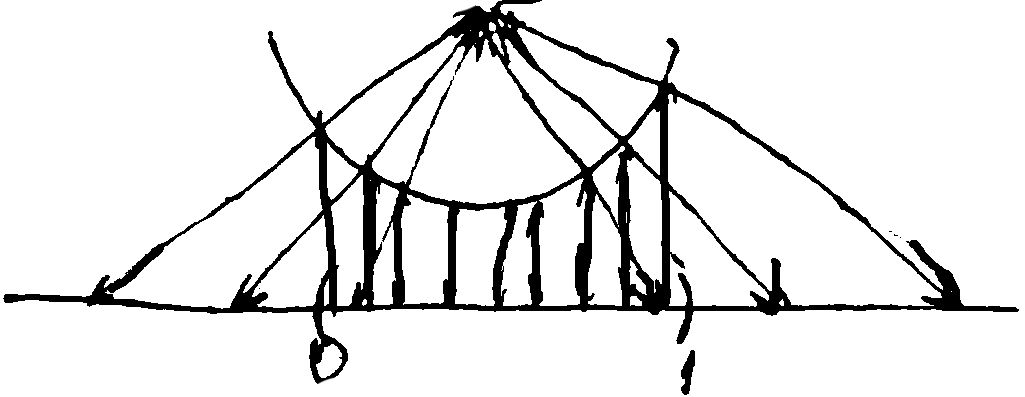
\includegraphics[scale=0.15]{d_ch_8_2}

        $(0, 1)$ эквивалентно $\mathbb{R}$

        $\mathbb{R}_{\textrm{несчет.}} = \mathbb{Q}_{\textrm{счет.}} \cup \overline{\mathbb{Q}} \Rightarrow \overline{\mathbb{Q}}$ несчетная.


    \section{Числовые последовательности и их пределы}
    
    \subsection{Числовые последовательности и их свойства}
    
    \textbf{Определение.} Пусть \(\forall n \in \mathbb{N}\) поставить в соответствие единственное число \(x_n \in \mathbb{R}\), тогда \(x_n\) --- числовая последовательность. То есть \(x_n\) --- отображение, заданное на множестве \(\mathbb{N}\).
    
    \subsubsection{Способы задания последовательностей}
    
    \begin{enumerate}
    	\item Формула n-го члена
        \item Рекуррентная формула
        \item Словесное задание
    \end{enumerate}
    
    \subsection{Понятие монотонности и ограниченности последовательности}
    
    \textbf{Определение.} Числовая последовательность называется
    \begin{itemize}
    	\item возрастающей, если \(\forall n \in \mathbb{N}\ x_n < x_{n+1}\)
        \item убывающей, если \(\forall n \in \mathbb{N}\ x_n > x_{n+1}\)
        \item неубывающей, если \(\forall n \in \mathbb{N}\ x_n \leq x_{n+1}\)
        \item невозрастающей, если \(\forall n \in \mathbb{N}\ x_n \geq x_{n+1}\)
  	\end{itemize}
    
    \textbf{Определение.} Монотонная последовательность – это неубывающая или невозрастающая последовательность.

    \textbf{Определение.} Числовая последовательность \(\{x_n\}\) называется ограниченной, если \(\exists M\ :\ \forall n \in \mathbb{N}\ \abs{x_n} \leq M\); ограниченна снизу, если \(\exists m\ :\ \forall n \in \mathbb{N}\ x_n \geq m\); ограниченна сверху, если \(\exists M_1\ :\ \forall n \in \mathbb{N}\ x_n \leq M_1\).
    
    \subsection{Арифметическая и геометрическая прогрессии}
    
    \subsubsection{Арифметическая прогрессия}
    
    \textbf{Определение.} Арифметической прогрессией конечной или бесконечной будем называть числовую последовательность, у которой каждый её член, начиная со второго, есть сумма предыдущего её члена и некоторого фиксированного числа.
    \\ \(x_{n+1} = x_n + d\); \(x_1\) --- задан, d --- разность арифметической прогрессии.
    
    \textbf{Свойства}
    
    \begin{enumerate}
    	\item Три числа \(x_{n-1}\), \(x_{n}\), \(x_{n+1}\) являются последовательными членами а.п. \(\Leftrightarrow\) \(x_n = \frac{x_{n-1} + x_{n+1}}{2}\)
        \item \(x_n = x_k + (n-k)*d\)\\
        \textit{Замечание.} \(x_n = x_1 + (n-1)*d\)\\
        \(\uparrow\ x_n = x_{n-1} + d = x_{n-2} + 2d = ... = x_1 + (n-1)*d \downarrow\).

        \item \(\begin{aligned}
            x_n = x_{n-k} + k*d \\
            x_{n+k} = x_n + k*d
        \end{aligned}
        ,\ k \in \mathbb{N} \Leftrightarrow 
        \begin{aligned}
            d = \frac{x_n - x_{n-k}}{k} \\
            d = \frac{x_{n+k} - x_n}{k}
        \end{aligned}
        \Leftrightarrow x_n - x_{n-k} = x_{n+k} - x_n \Leftrightarrow x_n = \frac{x_{n-k} + x_{n+k}}{2}\)

		\item \(x_k + x_l = x_m + x_n\), если \(k + l = m + n\)
        \\ \( \uparrow \) Пусть k --- самый маленький номер 
        \\ \(x_l = x_k + (l-k)d\\ x_m = x_k + (m - k)d\\ x_n = x_k + (n-k)d\)
        \\ левая часть = \(x_k + x_l = 2x_k + (l-k)d\)
        \\ правая часть = \(x_m + x_n = 2x_k + (m+n-2k)d = 2x_k + (l-k)d\ \downarrow\)

        \item \(S_n = \frac{(x_1 + x_n)n}{2}\)
        \\ \(\uparrow\) 
        \\ \(S_n = x_1 + x_2 + ... + x_n\)
        \\ \(+\)
        \\ \(S_n = x_n + x_{n-1} + ... + x_2 + x_1\)
        \\ \(\Downarrow\)
        \\ \(2S_n = (x_1 + x_n)n\)
        \\ \(S_n = \frac{(x_1 + x_n)n}{2} \downarrow\)
    \end{enumerate}
    
    \subsubsection{Геометрическая прогрессия}
    
    \textbf{Определение.} Геометрической прогрессией конечной или бесконечной назовём числовую последовательнность, у которой каждый член, начиная со второго, равен произведению предыдущего её члена на фиксированное для данной последовательности число \(q \not = 0\)
    \\ \(x_{n+1} = x_n * q\); \(x_1\) --- задан, \(x_1 \not = 0\), q --- множитель геометрической прогрессии
    
    \textbf{Свойства}
    
    \begin{enumerate}
    	\item Три последовательных числа \(x_{n-1},\ x_n,\ x_{n+1}\) являются членами одной геометрической прогрессии(в указанном порядке) \(\Leftrightarrow x_n^2 = x_{n-1}*x_{n+1}\)
        \\ \(\uparrow \begin{aligned}
				&x_{n+1} = x_n * q\\
				&x_n = x_{n-1} * q
			\end{aligned} \Leftrightarrow
            \begin{aligned}
				&q = \frac{x_{n+1}}{x_n}\\
				&q = \frac{x_{n}}{x_{n-1}}
			\end{aligned} \Leftrightarrow \frac{x_{n+1}}{x_n} = \frac{x_n}{x_{n-1}} \Leftrightarrow x_n^2 = x_{n-1} * x_{n+1} \downarrow\)
            
            \textbf{Замечание.} Если все \(x_n > 0,\ n \in \mathbb{N}\), тогда \(x_n = \sqrt{x_{n-1}*x_{n+1}}\)
        
        \item Получим формулу \(x_n\).
        \\ \(x_n = x_{n-1}*q = x_{n-2} * q^2 = ... = x_1 * q^{n-1}\\ x_n = x_1 * q^{n-1}\\ x_n = x_k * q^{n-k}\)

        \item \(\begin{aligned}
				&x_n = x_{n-k}*q^k\\
				&x_{n+k} = x_n*q^k
			\end{aligned} \Leftrightarrow
            \begin{aligned}
				&q^k = \frac{x_n}{x_{n-k}}\\
				&q^k = \frac{x_{n+k}}{x_n}
			\end{aligned} \Leftrightarrow x_n^2 = x_{n-k}*x_{n+k}\)
        
        \item \(x_k * x_l = x_m * x_n\), если \(k+l=m+n\)
        
        Пусть k --- самый маленький номер\\
        \(x_l = x_k q^{l-k}\\
        x_m = x_k q^{m-k}\\
        x_n = x_k q^{n-k}\)\\
        левая часть \(= x_k x_l = x_k^2 q^{l-k}\)\\
        правая часть \(= x_m x_n = x_k^2 q^{m + n - 2k} = x_k^2 q^{l + k - 2k} = x_k^2 q^{l-k}\)
        \item \(\begin{aligned}
        	&\quad S_n = x_1 + \cancel{x_1 q} + \cancel{x_1 q^2} + ... + \cancel{x_1 q^{n-1}}\\
            & -\\
            &\quad q S_n = \cancel{x_1 q} + \cancel{x_1 q^2} + \cancel{x_1 q^3} + ... + x_1 q^n
            \end{aligned} \Rightarrow (1-q)S_n = x_1 - x_1 q^n\)
            
            Если \(1 - q \not = 0 \Rightarrow S_n = \frac{x_1(1-q^n)}{1-q}\)\\
            Если \(1 - q = 0 \Rightarrow q = 1,\ S_n = n x_1\)
        \item \begin{enumerate}
        	\item Если \(q > 1\), то все \(x_n\) одного знака, \(\{x_n\}\) возрастает по абсолютной величине
            \item Если \(0 < q < 1\), то все \(x_n\) одного знака, \(\{x_n\}\) убывает по абсолютной величине
            \item Если \(q < -1\), то знаки последовательности чередуются, \(\{x_n\}\) возрастает по абсолютной величине
            \item Если \(-1 < q < 0\), то знаки последовательности чередуются, \(\{x_n\}\) убывает по абсолютной величине
            \item Если \(q = 1 \Rightarrow\) постоянна, \(\{x_n\} = x_1\)
            \item Если \(q = -1 \Rightarrow x_1, -x_1, x_1, -x_1, ...\)
        \end{enumerate}
    \end{enumerate}
    
    \subsection{Определение предела числовой последовательности}
    
    \textbf{Определение.} Будем говорить, что \( x_n \) сходится к \( a(\lim_{n \to \infty} x_n = a) \), если \( \forall \varepsilon > 0 \ \exists \  N = N(\varepsilon): \forall n > N,\ \abs{x_n - a} < \varepsilon \)
    
    \subsection{Геометрический смысл определения предела}
    
    a --- предел \( x_n \), \(a - \varepsilon < x_n < a + \varepsilon\)\\
	\(O_a = (a - \varepsilon,\ a + \varepsilon)\) --- \(\varepsilon\)-окрестность т. a

	
\includegraphics[scale=0.7]{21_0}
    
    \subsection{Теорема о единственности существующего предела}
    
    \textbf{Теорема 1.} Если \(\lim_{n \rightarrow \infty}{x_n} = a\), то \(a\ \exists !\)
    
    \(\uparrow\) От противного
    \\ Пусть \(\lim_{n \rightarrow \infty}{x_n} = a_1\) и \(\lim_{n \rightarrow \infty}{x_n} = a_2\), где \( a_1 < a_2\).
    
    Геометрический смысл:\\
    \(\forall \varepsilon > 0 \ \exists \  N_1 : n > N_1,\ a_1 - \varepsilon < x_n < a_1 + \varepsilon\\ \forall \varepsilon > 0 \ \exists \  N_2 : n > N_2,\ a_2 - \varepsilon < x_n < a_2 + \varepsilon
    \\ n > \max{(N_1, N_2)}\)
    
    \textit{Примечание.} Далее $U_{\varepsilon}(a)$ обозначается $\varepsilon$-окрестность $a$.

    Пусть \(\varepsilon < \frac{a_2 - a_1}{2} \Rightarrow U_{\varepsilon}(a_1)\ \cancel{\cap}\ U_{\varepsilon}(a_2)\), но такого быть не может, т.к. для \(n > \max{(N_1, N_2)}\
    \begin{aligned}
    	&x_n \in U_{\varepsilon}(a_1)\ \textrm{и}\\
        &x_n \in U_{\varepsilon}(a_2)
    \end{aligned}\) --- противоречие \(\downarrow\)
    
    \subsection{Теорема об ограниченности последовательности, имеющей предел}
    
    \textbf{Теорема 2.} Если \(\exists\ \lim_{n \rightarrow \infty}{x_n} = a\), то \(x_n\) --- ограничена
    
    \(\uparrow x_n\) --- ограничена(\(\forall n\ \exists\ M,\ \abs{x_n} < M\))?
    
    Дано: \(\forall \varepsilon > 0\ \exists\ N : \forall n > N,\ \abs{x_n - a} < \varepsilon\\ a - \varepsilon < x_n < a + \varepsilon\).
    
    Возьмём \(\varepsilon = \varepsilon_*\) такое, чтобы все члены \(x_n\) удовлетворяли \(a - \varepsilon_* < x_n < a + \varepsilon_*\),\\
    тогда \(M = \max{(\abs{a - \varepsilon_*}, \abs{a + \varepsilon_*})}\), т.е. \(x_n\) --- ограничена \(\downarrow\)
    
    \subsection{Теорема о сохранении знака (отделении от нуля)}
    
    \textbf{Теорема 3.} Пусть \(x_n\) --- сходится, т.е. \(\exists\ \lim_{n \rightarrow \infty}{x_n} = a,\ a \not = 0\), тогда \(\exists\ N_1 : \forall n > N_1,\ \abs{x_n} > \frac{\abs{a}}{2}\ (*)\)
    
    В частности \(\begin{aligned}
    	&a > 0 \quad x_n > \frac{a}{2} > 0\ (1)\\
        &a < 0 \quad x_n < \frac{a}{2} < 0\ (2)
    \end{aligned}\)
    
    \(\uparrow\) Дано: \(\forall \varepsilon > 0\ \exists\ N(\varepsilon) : \forall n > N,\ \abs{x_n - a} < \varepsilon\) или \(a - \varepsilon < x_n < a + \varepsilon\)
    
    Пусть \(\varepsilon = \frac{\abs{a}}{2} > 0 \Rightarrow a - \frac{\abs{a}}{2} < x_n < a + \frac{\abs{a}}{2}\)
    \begin{enumerate}
    	\item Если \(a > 0 \Rightarrow 0 < \frac{a}{2} < x_n < \frac{3a}{2}.\ N_1 = N\)
        \item Если \(a < 0 \Rightarrow \frac{3a}{2} < x_n < a - \frac{a}{2} = \frac{a}{2} < 0.\ N_1 = N\)
    \end{enumerate}
    
    В общем случае \(\abs{x_n - a} < \frac{\abs{a}}{2}\)
    
    \[\abs{a + b} \leq \abs{a} + \abs{b}\]
    \[\abs{a} = \abs{a - b + b} \leq \abs{a - b} + \abs{b}\]
    \[\Downarrow\]
    \[\underline{\abs{a} - \abs{b} \leq \abs{a - b}}\]
    \[\abs{b} = \abs{b - a + a} \leq \abs{b - a}(= \abs{a - b}) + \abs{a}\]
    \[\Downarrow\]
    \[\underline{\abs{b} - \abs{a} \leq \abs{a - b}}\ (*)\]
    \[-\abs{a-b} \leq \abs{a} - \abs{b} \leq \abs{a - b}\]
    \[\Downarrow\]
    \[\underline{\abs{\abs{a} - \abs{b}} \leq \abs{a - b}}\ (**)\]
    
    По $(*):$

    \(\abs{a} - \abs{x_n} \leq \abs{x_n - a} < \frac{\abs{a}}{2}\\ \frac{\abs{a}}{2} < \abs{x_n}\ \downarrow\)
    
    \textbf{Теорема 4.} Если \(\lim_{n \rightarrow \infty}{x_n} = a\), то \(\lim_{n \rightarrow \infty}{\abs{x_n}} = \abs{a}\)
    
    \(\uparrow\) Дано: \(\forall \varepsilon > 0\ \exists\ N : \forall n > N,\ \abs{x_n - a} < \varepsilon\)
    
    По $(**):$

    \(\abs{\abs{x_n} - \abs{a}} \leq \abs{x_n - a} < \varepsilon\)
    
    Получилось \(\forall \varepsilon > 0\ \exists\ N : \forall n > N,\ \abs{\abs{x_n} - \abs{a}} < \varepsilon\) --- определение \(\lim_{n \rightarrow \infty}{\abs{x_n}} = \abs{a}\ \downarrow\)

    \subsection{Теорема о пределе последовательности, полученной сдвигом нумерации}
    
    \textbf{Теорема 5.} \(\lim_{n \rightarrow \infty}{x_n} = a\), тогда \(\lim_{n \rightarrow \infty}{x_{n+k}} = a\)
    
    \(\uparrow\) Дано: \(\forall \varepsilon > 0\ \exists\ N : \forall n > N,\ \abs{x_n - a} < \varepsilon\)
    
    Надо: \(\forall \varepsilon > 0\ \exists\ N_1 : \forall n > N_1,\ \abs{x_{n+k} - a} < \varepsilon\)
    
    \(n' = n + k\ n' > N\) всё хорошо
    \\ \(n + k > N\\ n > N - k\), т.е. \(N_1 = N - k\ \downarrow\)
    
    \subsection{Теорема о предельном переходе в неравенствах}
    
    \textbf{Теорема 6.} Пусть \(x_n \xrightarrow[n \rightarrow \infty]{} a;\ y_n \xrightarrow[n \rightarrow \infty]{} b\) и \(\forall n\ x_n \leq y_n \Rightarrow a \leq b\)
    
    \(\uparrow\) Дано: \(\forall \varepsilon > 0\ \begin{aligned}
    	&\exists\ N_1 : \forall n > N_1,\ a - \varepsilon < x_n < a + \varepsilon
        &\exists\ N_2 : \forall n > N_2,\ b - \varepsilon < y_n < b + \varepsilon
        \end{aligned}\)
    
    От противного. Пусть \(b < a\). Возьмём \(\varepsilon = \frac{a-b}{2}\); и \(n > \max{(N_1, N_2)}\).
    
    Тогда \(y_n \leq b + \varepsilon = b + \frac{a-b}{2} = \frac{a + b}{2} = a - \frac{a-b}{2} = a - \varepsilon < x_n\) --- противоречие \(\downarrow\)
    
    \textbf{Замечание.} Если \(\forall n\ x_n < y_n \xrightarrow[n \rightarrow \infty]{} a \leq b\)
  
    \textbf{Следствие.} Если \(x_n \xrightarrow[n \rightarrow \infty]{} a,\ \forall n\ x_n \in [c,\ d] \Rightarrow a \in [c,\ d]\)
    
    \(\uparrow\) Пусть \(c_n = c,\ d_n = d\ \forall n\ c_n \leq x_n \leq d_n \xrightarrow[n \rightarrow \infty]{} c \leq a \leq d \Rightarrow a \in [c,\ d]\ \downarrow\)
    
    \subsection{Теорема о двух милиционерах}
    
    \textbf{Теорема 7.} Пусть \(\begin{aligned}
    	&x_n \xrightarrow[n \rightarrow \infty]{} a\\
        &y_n \xrightarrow[n \rightarrow \infty]{} a
        \end{aligned}\) и \(\forall n\ x_n \leq z_n \leq y_n\), тогда \(\exists\ \lim_{n \rightarrow \infty}{z_n} = a\)
        
    \(\uparrow\) Дано: \(\forall \varepsilon > 0\ \begin{aligned}
    	&\exists\ N_1(\varepsilon) : \forall n > N_1,\ a - \varepsilon < x_n < a + \varepsilon\\
        &\exists\ N_2(\varepsilon) : \forall n > N_2,\ a - \varepsilon < y_n < a + \varepsilon
    	\end{aligned}\)
    
    \(\forall n > \max{(N_1, N_2)},\ a - \varepsilon < x_n \leq z_n \leq y_n < a + \varepsilon\), т.е. \(z_n \xrightarrow[n \rightarrow \infty]{} a\ \downarrow\)
    
    \subsection{Теорема о сумме, разности, произведении и частном пределов}
    
    \textbf{Определение.} Пусть существуют конечные пределы $\lim_{n \rightarrow \infty}{x_n} = a$ и $\lim_{n \rightarrow \infty}{y_n} = b$ числовых последовательностей $\{x_n\}$ и $\{y_n\}$. Тогда существуют пределы суммы, разности и произведения последовательностей, которые равны, соответственно, сумме, разности и произведению их пределов. Если  $b \neq 0$  и  $y_n \neq 0$  для всех $n$, то существует предел частного последовательностей, равный частному пределов.

    \textbf{Теорема 8.} Пусть \(\begin{aligned}
    	\lim_{n \rightarrow \infty}{x_n} = a\\
        \lim_{n \rightarrow \infty}{y_n} = b
        \end{aligned}\), то
        \begin{enumerate}
        	\item \(\lim_{n \rightarrow \infty}{x_n \pm y_n} = a \pm b\)
            \item \(\lim_{n \rightarrow \infty}{x_n y_n} = a*b\)
            \item \(\lim_{n \rightarrow \infty}{\frac{x_n}{y_n}} = \frac{a}{b} \quad,\ b \neq 0,\ \forall n\ y_n \neq 0\)
        \end{enumerate}
    
    \(\uparrow\) Дано: \(\begin{aligned}
      	&\forall \varepsilon_1 > 0\ \exists\ N_1 : \forall n > N_1,\ \abs{x_n - a} < \varepsilon_1\\
        &\forall \varepsilon_2 > 0\ \exists\ N_2 : \forall n > N_2,\ \abs{y_n - a} < \varepsilon_2
        \end{aligned}\)
    
    \begin{enumerate}
    	\item Надо: \(\forall \varepsilon > 0\ \exists\ N(\varepsilon) : \forall n > N,\ \abs{x_n + y_n - (a+b)} < \varepsilon\)
        
        \(\abs{x_n + y_n - (a+b)} = \abs{x_n - a + y_n - b} \leq \abs{x_n - a} + \abs{y_n - b} < \varepsilon_1 + \varepsilon_2 = \varepsilon\).
        
        \(\varepsilon \rightarrow \varepsilon_1,\ \varepsilon_2 \rightarrow N_1,\ N_2 \rightarrow N = \max{(N_1, N_2)}\)
        
        \item Надо: \(\forall \varepsilon > 0\ \exists\ N(\varepsilon) : \forall n > N,\ \abs{x_n y_n - a*b} < \varepsilon\)
        
        \(\abs{x_n y_n - a*b} = \abs{x_n y_n - a*y_n + a*y_n - a*b} \leq \abs{y_n} \abs{x_n - a} + \abs{a} \abs{y_n - b} \underset{\exists\ M : \abs{y_n} < M} < \abs{y_n} \varepsilon_1 + \abs{a} \varepsilon_2 < M \varepsilon_1 + \abs{a} \varepsilon_2 = \varepsilon\\
        \varepsilon \rightarrow \varepsilon_1 = \frac{\varepsilon}{2M},\ \varepsilon_2 = \frac{\varepsilon}{2 \abs{a}} \rightarrow N_1,\ N_2 \rightarrow N = \max{(N_1, N_2)}\)
        
        \item Надо: \(\forall \varepsilon > 0\ \exists\ N : \forall n > N,\ \abs{\frac{x_n}{y_n} - \frac{a}{b}} < \varepsilon\)
        
        \(\abs{\frac{x_n}{y_n} - \frac{a}{b}} = \abs{\frac{x_n b - y_n a}{y_n b}} = \frac{\abs{x_n b - y_n a}}{\abs{b} \abs{y_n}} = \frac{\abs{x_n b - a*b + a*b - y_n a}}{\abs{b} \abs{y_n}} \leq \frac{\abs{b} \abs{x_n - a}}{\abs{b} \abs{y_n}} +
        \frac{\abs{a} \abs{y_n - b}}{\abs{b} \abs{y_n}} < \frac{\varepsilon_1}{y_n} + \frac{\abs{a}}{\abs{b} \abs{y_n}} \varepsilon_2\)
        
        По теореме 3 \(\exists\ N_3 : \forall n > N_3,\ \abs{y_n} > \frac{\abs{b}}{2} \Rightarrow \frac{1}{\abs{y_n}} < \frac{2}{\abs{b}}\)
        
        \(\frac{\varepsilon_1}{y_n} + \frac{\abs{a}}{\abs{b} \abs{y_n}} \varepsilon_2 < \frac{2 \varepsilon_1}{b} + \frac{2 \abs{a}}{\abs{b}^2} \varepsilon_2 = \varepsilon\\ N = \max{(N_1, N_2, N_3)}\ \downarrow\)
    \end{enumerate}
    
    \subsection{Бесконечно малые последовательности и их свойства}
    
    \textbf{Определение.} Числовая последовательность \(\alpha_n\) называется бесконечно малой, если \(\lim_{n \rightarrow \infty}{\alpha_n} = 0\). \(\forall \varepsilon > 0\ \exists\ N : \forall n > N,\ \abs{\alpha_n} < \varepsilon\)
    
    \textbf{Свойства}
    
    \begin{enumerate}
    	\item Сумма конечного числа бесконечно малых есть величина бесконечно малая
        \item Разность двух бесконечно малых --- бесконечно малая ч.п.
        \item \(\alpha_n\) --- б.м.; \(\beta_n\) ограничена \(\Rightarrow \alpha_n \beta_n\) --- б.м.
        
        \(\uparrow\) Надо: \(\lim_{n \rightarrow \infty}{\alpha_n \beta_n} = 0\), т.е. \(\forall \varepsilon > 0\ \exists\ N : \forall n > N,\ \abs{\alpha_n \beta_n} < \varepsilon\)
        
        Дано: \(\forall \varepsilon_1 > 0\ \exists\ N_1 : \forall n > N_1,\ \abs{\alpha_n} < \varepsilon_1;\ \forall n\ \abs{\beta_n} < M\)
        
        \(\abs{\alpha_n \beta_n} = \abs{\alpha_n} \abs{\beta_n} < \varepsilon_1 M = \varepsilon\\ \varepsilon_1 = \frac{\varepsilon}{M},\ N = N_1\ \downarrow\)
        
        \item \(\lim_{n \rightarrow \infty}{x_n} = a \Leftrightarrow x_n = a + \alpha_n\), где \(\alpha_n\) --- б.м.
        
        \(\uparrow\ \lim_{n \rightarrow \infty}{x_n} = a \Rightarrow \lim_{n \rightarrow \infty}{(x_n - a)} = 0 \Rightarrow \alpha = x_n - a\) --- б.м. \(\Rightarrow x_n = a + \alpha_n\), где \(\alpha_n\) --- б.м.
        
        \(``\Leftarrow" x_n = a + \alpha_n\), где \(\alpha_n\) --- б.м. \(\Rightarrow \lim_{n \rightarrow \infty}{x_n} = \lim_{n \rightarrow \infty}{(a + \alpha_n)} = a\ \downarrow\)
    \end{enumerate}
    
    \subsection{Пределы \(q^n,\ \sqrt[n]{a},\ \sqrt[n]{n}\)}
    
    \subsubsection{Предел \(q^n\)}
    
    \(\lim_{n \rightarrow \infty}{q^n} = 0\), если \(\abs{q} < 1\)
        
        \begin{enumerate}
        	\item Если \(q = 0\), то очевидно
            
            \item Если \(q \not = 0\)
            
            \(\uparrow\) Надо: \(\forall \varepsilon > 0\ \exists\ N : \forall n > N,\ \abs{q^n} < \varepsilon
            \\ q \not = 0 \Rightarrow \frac{1}{\abs{q}} > 1 \Rightarrow \frac{1}{\abs{q}} = 1 + \alpha,\ \alpha > 0\\
            \frac{1}{\abs{q}^n} = (1 + \alpha)^n > \alpha n\\ \Downarrow\\ \abs{q}^n < \frac{1}{\alpha n}\)
            
            \(\abs{q^n} = \abs{q}^n < \frac{1}{\alpha(> 0) n} < \varepsilon\\ n > \frac{1}{\alpha \varepsilon}\)
            
            \(N = [\frac{1}{\alpha \varepsilon}] + 1\ \downarrow\)
        \end{enumerate}
        
    \subsubsection{Предел \(\sqrt[n]{a}\)}
        
        \(\lim_{n \rightarrow \infty}{\sqrt[n]{a}} = 1\)
        \begin{enumerate}
        	\item Если \(a = 1\), то очевидно
            
            \item Если \(a > 1 \Rightarrow \sqrt[n]{a} > \sqrt[a]{1} = 1 \Rightarrow\\
            \Rightarrow \sqrt[n]{a} = 1 + \alpha_n,\ \alpha_n > 0\).
            
            \(a = (1 + \alpha_n)^n > \alpha_n n \Rightarrow \alpha_n < \frac{a}{n}\\
            0(\rightarrow 0) < \alpha_n < \frac{a}{n}(\rightarrow 0)\), по Т. о 2х милиционерах \(\lim_{n \rightarrow \infty}{\alpha_n} = 0 \Rightarrow \lim_{n \rightarrow \infty}{\sqrt[n]{a}} = 1\)
            
            \item \(0 < a < 1 \Rightarrow \frac{1}{a} > 1\)
            
            \(\lim_{n \rightarrow \infty}{\sqrt[n]{a}} = \lim_{n \rightarrow \infty}{\frac{1}{\sqrt[n]{\frac{1}{a}}}} = \frac{\lim_{n \rightarrow \infty}{1}}{\lim_{n \rightarrow \infty}{\sqrt[n]{\frac{1}{a}}}}
            = \frac{1}{1} = 1\)
        \end{enumerate}
        
    \subsubsection{Предел \(\sqrt[n]{n}\)}
        
        \(\lim_{n \rightarrow \infty}{\sqrt[n]{n}} = 1\)
        
        \(\sqrt[n]{n} \geq \sqrt[n]{1} = 1 \Rightarrow\\
        \Rightarrow \sqrt[n]{n} = 1 + \alpha_n,\ \alpha_n > 0\)
        
        \(n = (1 + \alpha_n)^n = 1 + \alpha_n n + c_n \alpha_n^2 + ... = 1 + \alpha_n n + \frac{n(n-1)}{2} \alpha_n^2 + ...
        \underset{\textrm{``выбрасываем'' все слагаемые, кроме} \frac{n(n-1)}{2} \alpha_n^2} > \frac{n(n-1)}{2} \alpha_n^2 \Rightarrow 0 < \alpha_n^2 < \frac{2 \not n}{\not n (n-1)} \Rightarrow\)
        \[\Rightarrow 0(\rightarrow 0) < \alpha_n < \frac{\sqrt{2}}{\sqrt{n-1}}(\rightarrow 0) \Rightarrow\]
        \(\Rightarrow\) по Т. о 2х милиционерах \(\lim_{n \rightarrow \infty}{\alpha_n} = 0 \Rightarrow \lim_{n \rightarrow \infty}{\sqrt[n]{n}} = 1\ \downarrow\)
    
    
    \subsection{Сумма членов бесконечно убывающей геометрической прогрессии}
    
    \(S = b + b q + b q^2 + ... + b q^n + ...\\
    \abs{q} < 1\)
    
    \(S_n = b + b q + b q^2 + ... + b q^{n-1} = \frac{b(1 - q^n)}{1 - q}\)
    
    \(\lim_{n \rightarrow \infty}{S_n} = \lim_{n \rightarrow \infty}{\frac{b(1 - q^n)}{1 - q}} = \frac{b}{1 - q} \lim_{n \rightarrow \infty}{(1 - q^n)} = \frac{b}{1 - q}\)
    
    \subsection{Бесконечно большие и расходящиеся последовательности и их свойства}
    
    \textbf{Определение.} Если \(x_n\) не является сходящейся, то она называется расходящейся
    
    \textbf{Определение.} Числовая последовательность \(x_n\) называется бесконечно большой, если \(\forall E > 0\ \exists\ N : \forall n > N,\ \abs{x_n} > E\)
    
    \textbf{Определение.} \(\lim_{n \rightarrow \infty}{x_n} = +\infty;\ \forall E > 0\ \exists\ N : \forall n > N,\ x_n > E\)
    
    \textbf{Определение.} \(\lim_{n \rightarrow \infty}{x_n} = -\infty;\ \forall E > 0\ \exists\ N : \forall n > N,\ x_n < -E\)
    
    \textbf{Теорема.} Если \(\alpha_n\) --- б.м. \(\Leftrightarrow \frac{1}{\alpha_n}\) --- б.б.
    
    \(\uparrow\ \alpha_n\) --- б.м.\\
    \(\forall \varepsilon > 0\ \exists\ N_1 : \forall n > N_1,\ \abs{\alpha_n} < \varepsilon\)
    
    \(\beta_n = \frac{1}{\alpha_n}\) --- б.б.\\
    \(\forall E > 0\ \exists\ N_2 : \forall n > N_2,\ \frac{1}{\abs{\alpha_n}} > E\)
    
    \(``\Rightarrow" \frac{1}{\abs{\alpha_n}} > \frac{1}{\varepsilon} = E;\ \varepsilon = \frac{1}{E}\\
    E \rightarrow \varepsilon \rightarrow N_1 \rightarrow N_2 = N_1\)
    
    \(``\Leftarrow" \abs{\alpha_n} > \frac{1}{E} = \varepsilon\\
    \varepsilon \rightarrow E = \frac{1}{\varepsilon} \rightarrow N_2 \rightarrow N_1 = N_2\ \downarrow\)
    
    \subsubsection{Свойства бесконечно больших числовых последовательностей}
    
    \begin{enumerate}
        \item Если \( \lim_{n \rightarrow \infty }a_n = + \infty\ (+\infty + c) \), а \( \{b_n\} \) ограничена снизу, т.е. \( b_n \geq b\ \forall n \), тогда \(\lim_{n \rightarrow \infty}{(a_n + b_n)} = +\infty\)
       
        \item Если \( \lim_{n \rightarrow \infty }a_n = + \infty\ (+\infty * c) \), а \( \{b_n\} \) ограничена снизу \( M: b_n \geq M > 0\ \forall n,\ \lim_{n \rightarrow \infty}{(a_n * b_n)} = +\infty\)

        \item Если \( \lim_{n \rightarrow \infty }a_n = +\infty \), а \( b_n \) ограничена, т.е. \( 0 < b_n < M (n \rightarrow \infty)\ \forall n \), то \[ (\frac{+\infty}{c > 0}) \lim_{n \rightarrow \infty}{\frac{a_n}{b_n}} = +\infty\]
    
        \item Если \(\lim_{n \rightarrow \infty}{a_n} = \infty\), а \(b_n\) ограничена: \(\abs{b_n} \leq M\  \forall n\), \[ (\frac{M}{\infty}) \lim_{n \rightarrow \infty }\frac{b_n}{a_n} = 0\]
    \end{enumerate}
    
    \subsection{Неопределенности (понятие)}
    
    \textbf{Определение.} Предел последовательности, значение которого не может быть однозначно определено, называется неопределённостью

    \begin{enumerate}
    	\item \(\{\infty - \infty\}\)
    	
    	\(2n - n = n \rightarrow +\infty\)
    	
        \(\lim_{n \rightarrow \infty}{\sqrt{n+1} - \sqrt{n}} = \lim_{n \rightarrow \infty}{\frac{n+1-n}{\sqrt{n+1}+\sqrt{n}}}\) = 0

    	\item \(\{\frac{\infty}{\infty}\}\)

    	\( n^2,\ n,\ 2n \)
    
    	\( \frac{n^2}{n}  \rightarrow +\infty;\ \frac{n}{n^2} \rightarrow 0\)

    	\item \(\{\infty * 0\}\)
    	\item \(\{\frac{0}{0}\}\)
    	
    	% \(\lim_{n \rightarrow \infty}{a_n}\)
    	\item \(\{1^{\infty}\}\)
    	\item \(\{0^0\}\)
    	\item \(\{\infty^0\}\)
    \end{enumerate}
    
    \subsection{Стабилизирующиеся последовательности}
    
    \textbf{Определение.}
    Числовая последовательность целых чисел называется стабилизирующейся к \(\xi\), если \( \exists\ n_0 : \forall n > n_0\  a_n = \xi\), то есть \(a_n \rightrightarrows \xi \)
    
    \subsubsection{Лемма 1}
    
    Если \(\{a_n\}\) --- последовательность целых неотрицательных чисел, неубывающая и ограниченная сверху, т.е. \( a_n \leq M\ \forall n\), то \( \exists\ \xi: a_n \rightrightarrows \xi \) и \( \xi \leq M \).

    \(\uparrow\)

    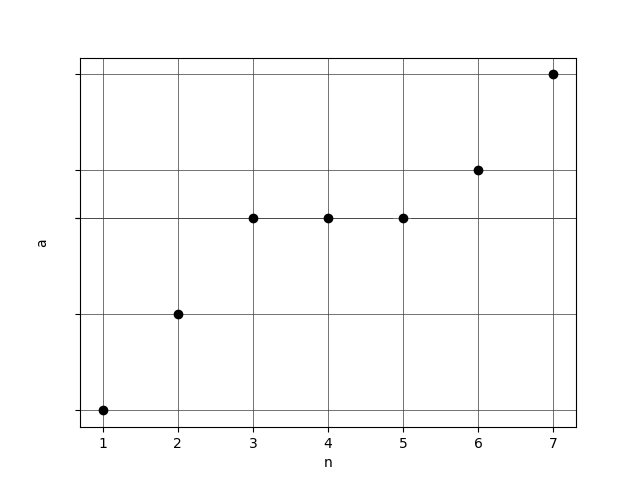
\includegraphics[scale=0.6]{8}
    
    хотя число членов последовательности \(\infty\), но между \(a_1\) (самый маленький член последовательности т.к. \( a_n \not\searrow \)) и \(M\) есть только конечное число целых чисел, \(\Rightarrow\) только конечное число значений \(a_n\)\\
    Обозначим наибольшее значение принимаемое \( a_n \), ч/з \( \xi \), т.е. \( \exists n_0: a_{n_0} = \xi \leq M \), тогда \( \forall n > n_0\ a_n = \xi \), т.к. \( a_n \not \searrow\ \downarrow \)
    
    Рассмотрим $\{a_n\}$ --- последовательность б.д.д. Обозначим следующую таблицу (*)

    \(
      a_1 = \alpha_{10},\alpha_{11},\alpha_{12},\alpha_{13}...\\
      a_2 = \alpha_{20},\alpha_{21},\alpha_{22},\alpha_{23}...\\
      a_3 = \alpha_{30},\alpha_{31},\alpha_{32},\alpha_{33}...\\
      .\\
      .\\
      .\\
      .\\
      a_n = \alpha_{n0},\alpha_{n1},\alpha_{n2},\alpha_{n3}...\\
      -----------\\
      a = \gamma_{0},\gamma_{1},\gamma_{2},\gamma_{3}...
    \)

    \textbf{Определение.} Будем говорить, что последовательность б.д.д. \( (>0)\ \{a_n\} \rightrightarrows \)\\
    \( a = \gamma_0,\gamma_1\gamma_2\gamma_3...\ (a_n \rightrightarrows a) \), если \(\forall k \ \alpha_{nk} \rightrightarrows \gamma_k\)

    \subsubsection{Лемма 2}
    
    \(\{a_n\}\) --- б.д.д. >  0

    Если \( \{a_n\} \) --- последовательность неотрицательных б.д.д. (*) является неубывающей и ограниченной (т.е. \( \exists M \) (б.д.д., не оканчивающася последовательностью 9-ок)): \( \forall\ n\ a_n \leq M) \), то \( \exists\ a \):
    
    \begin{enumerate}
    	\item \(a_n \rightrightarrows\ a\)  

    	\item \(a_n \leq a \leq M\)
	\end{enumerate}
    
    \( \uparrow \) В табл. (*) cмотрим на первый столбец

    \( \alpha_{10} \)\\
    \( \alpha_{20} \)\\
    \( \alpha_{30} \)\\
    ...\\
    \( \alpha_{n0} \)

    Это последовательность неубывающих целых неотр. чисел и ограниченных сверху \(M\) по \textbf{Л1}\\
    \(\exists \) номер \(N_0\) \: \(\forall\ n > N_0\)\\
    \(\ \alpha_{n_0} \rightrightarrows\ \gamma_0\)
    
    \( \alpha_{10} \)\\
    \( \alpha_{20} \)\\
    \( \alpha_{30} \)\\
    ...\\
    \( \alpha_{N_00} = \gamma_0 \)\\
    \(\gamma_0\)\\
    \(\gamma_0\)

    Пусть \(n > N_1\), тогда смотрим на \(\{\alpha_{n1}\}\)

    \(\alpha_{n1}\) --- последовательность целых, неотр. чисел. Она ограничена 9-кой; неубывающая(т.к. \(a_n \not\searrow\) и 0-й столбец уже застабилиз.) \(\Rightarrow \ \exists\ N_1 \ \alpha_{n_1} \rightrightarrows\ \gamma_1 \ \forall n > N_1 \geq N_0\)

    Пусть \( n > N_1 \geq N_0 \) и смотрим \( \{ \alpha_{n2} \} \)
    
    \(\{\alpha_{n2}\}\) --- последовательность целых, неотр. чисел. Она ограничена 9-кой, неубывающей(т.к. \(a_n \not\searrow\) и 1-ый столбец уже застабилиз.) \(\Rightarrow \ \exists N_2 \ \: \ \forall n > N_2 \geq N_1 \geq N_0 \ \alpha_{n2} \rightrightarrows\ \gamma_2\) и т.д.

    в итоге \( \forall\ n > N_k \geq N_{k-1} \geq ... \geq N_0\quad \{ \alpha_{nk} \} \rightrightarrows\ \gamma_k \), то \( a_n \rightrightarrows\ a = \gamma_0,\gamma_1\gamma_2\gamma_3...\gamma_k... \)
    
    Из построения \(a_n \leq a \)
    \\ Осталось показать, что a \(\leq\) M

    Будем доказывать от противного: т.е. пусть \(a > M\), т.е. \(a_{(k)} = \gamma_0,\ \gamma_1,\ \gamma_2,\ ...,\ \gamma_k > M\)
    \\ \(a_k\) --- прибл. по недост. для a, но тогда \(a_n \ \: \ n > N_k\)
    \\ \(a_n = \alpha_{n0},\ \alpha_{n1},\ \alpha_{n2},\ ...,\ \alpha_{nk},\ \alpha_{nk+1},\ ... = \gamma_0,\ \gamma_1,\ ...,\ \gamma_k\alpha_{nk+1} > a_{(k)} > M\), противоречие с тем, что \(a_n \leq M \ \forall n \ \downarrow\)
    
    \subsection{Теорема Вейерштрасса}
    
    Если \(\{ x_n \} \) --- числовая последовательность неубывает и ограничена сверху, то она сходится.

    \(\uparrow\)
    \begin{enumerate}
        \item Пусть \( x_1 > 0 \Rightarrow \forall\ n\ x_n > 0 \) т.к. \( (x_n \not\searrow ) \).

        \item Любое \( x_n \in \mathbb{R} \) представлена в виде б.д.д.

        \item По \textbf{Л2}, такая (1) \( x_n \rightrightarrows a \)

        \item Покажем, что \(x_n \longrightarrow_{n \rightarrow \infty} a\)
    \\ Надо \(\forall \varepsilon > 0 \ \exists N \ \: \ \forall n > N\), \(\abs{x_n - a} < \varepsilon\)

    пусть \( n > N_k \), где \( N_k \) - номер, когда \(k\)-ый столбец в (*) застабилиз., тогда 
    \[ \abs{x_n - a} = \abs{\gamma_0,\gamma_1....\gamma_k\alpha_{nk+1}\alpha_{nk+2}... - \gamma_0,\gamma_1\gamma_2...\gamma_k\gamma{k+1}\gamma_{k+2}...} \]
    \[ = 0,\underbrace{0...0}_k\beta_{k+1}\beta_{k+2}... < 0,\underbrace{0...0}_{k-1}1 = \frac{1}{10^k} < \frac{1}{9k} < \varepsilon \]
    \[k > \frac{1}{9\varepsilon}\quad \varepsilon \rightarrow k \rightarrow N_k = N \downarrow \]
    \end{enumerate}

    \textbf{Замечание 1.} 
    Если \(x_1 < 0\), тогда рассм. \(y_1 = x_1 + c\ : \ y_1 > 0\), тогда по доказ. \( y_n = x_n + c \not\searrow \), ограничена сверху и \( y_1 > 0 \Rightarrow \) по доказ \(y_n \xrightarrow[n \rightarrow \infty]{} b\ \Rightarrow x_n \xrightarrow[n \rightarrow \infty]{} b - c\)
    
    \textbf{Замечание 2.}
    Аналогично можно доказать, что, если \(\{x_n\} \bcancel{\nearrow}\) и ограничена снизу, то она сх-ся.
    
    В общем случае:
    \\ Если последовательность монотонна и ограничена, то она сх-ся \(\downarrow\)
    
    \subsection{Число e (задание)}
    
    \begin{enumerate}
    	\item \( \{ x_n \} \) --- ограничена
    	\item \( \{ x_n \} \) --- монотонна
    \end{enumerate}
    
    Из 1) и 2) \( \Rightarrow \) сходятся

    \textbf{I монотонна и возрастает}

    \((a+b)^n = \sum_{k=0}^n\ C^k_n \ a^{n-k}b^k=1*a^n+\sum_{k=1}^n\ C^k_n \ a^{n-k}b^k = a^n+\sum_{k=1}^n \frac{n!}{k!(n-k)!} a^{n-k}b^k = \)

    \( = a^n + \sum_{k=1}^n \frac{n(n-1)(n-2)...(n-(k-1))}{k!} a^{n-k} b^k\)

    \( x_n = 1 + \sum_{k=0}^n \frac{n(n-1)(n-2)...(n-(k-1))}{k!} \frac{1}{n^k} = 1 + \frac{1}{1!} \frac{n}{n} + \frac{1}{2!} \frac{n(n-1)}{n^2} + \frac{1}{3!} \frac{n(n-1)(n-2)}{n^3} + ... + \)

    \( + \frac{1}{k!} \frac{n(n-1)...(n-(k-1))}{n^k} + ... + \frac{1}{n!} \frac{n(n-1)...(n-(n-1))}{n^n} = 1 + 1 + \frac{1}{2!} \frac{n-1}{n} + \frac{1}{3!} \frac{(n-1)(n-2)}{n^2} + ... + \frac{1}{k!} \frac{(n-1)(n-2)...(n-(k-1))}{n^{k-1}} + ... +\)

    \(x_n = 1+1+\frac{1}{2!}(1-\frac{1}{n})+\frac{1}{3!}(1-\frac{1}{n})(1-\frac{2}{n})+...+\frac{1}{k!}(1-\frac{1}{n})(1-\frac{2}{n})...(1-\frac{k-1}{n}) + ... + \frac{1}{n!} (1 - \frac{1}{n})(1 - \frac{2}{n})(1 - \frac{n-1}{n})\)

    \((a+b)^{n+1} = \sum_{k=0}^{n+1}\ C_{n+1}^k a^{n+1-k} b^k = a^{n+1} + \sum_{k=1}^{n+1} \frac{(n+1)n(n+1-2)...(n+1-(k-1))}{k!} a^{n+1-k} b^k\)

    \(x_{n+1} = 1 + 1 + \frac{1}{2!}(1-\frac{1}{n+1}) + \frac{1}{3!}(1-\frac{1}{n+1})(1-\frac{2}{n+1})+...+\frac{1}{k!}(1-\frac{1}{n+1})(1-\frac{2}{n+1})...(1-\frac{k-1}{n+1})+...\)\\
    \(...+\frac{1}{n!}(1-\frac{1}{n+1})(1-\frac{2}{n+1})...(1-\frac{n-1}{n+1}) + \underbrace{\frac{1}{(n+1)!}(1-\frac{1}{n+1})(1-\frac{2}{n+1})...(1-\frac{n}{n+1})}_{> 0}\)\\

    \(\frac{1}{n} > \frac{1}{n+1}\)

    \(-\frac{1}{n} < -\frac{1}{n+1}\)

    \(0 < (1-\frac{1}{n}) < (1-\frac{1}{n+1})\ n > 1\) 
    \\аналог: \\\(0 < 1-\frac{2}{n} < 1-\frac{2}{n+1} \Rightarrow (1-\frac{1}{n})(1-\frac{2}{n}) < (1 - \frac{1}{n+1})(1 - \frac{2}{n+1})\)
    
    Сравним \(x_n\) и \(x_{n+1}\) почленно
    
    \(\forall n \ x_n < x_{n+1} \Rightarrow\) возрастает

    \textbf{II ограничена}

    \( 2 < x_n < 2 + \frac{1}{2!} + \frac{1}{3!} + \frac{1}{4!} + ... + \frac{1}{k!} + ... + \frac{1}{n!} <\\
    < 2 + \frac{1}{2} + \frac{1}{2^2} + \frac{1}{2^3} ... \frac{1}{2^{k+1}}+...+\frac{1}{2^{n-1}} = 2 + \frac{\frac{1}{2} - \frac{1}{2^n}}{1 - \frac{1}{2}} = 2 + \frac{\not\frac{1}{2}(1-\frac{1}{2^{n-1}})}{\not\frac{1}{2}} = 3 - \frac{1}{2^{n-1}} < 3\)

    \( \frac{1}{1*2} = \frac{1}{2} \)

    \( \frac{1}{2*3} < \frac{1}{2*2} = \frac{1}{2^2} \)

    \( \frac{1}{3*4} < \frac{1}{2*2*2} = \frac{1}{2^3} \)

    \( x_n \nearrow \)\\
    \(\underbracket{2 < x_n < 3}_{\Downarrow} \)\\
    по теореме Вейерштрасса:\\
    \( \exists\ \lim_{n \rightarrow \infty} (1 + \frac{1}{n})^n = e \)
    \\\(e \approx 2.718281828459045...\)

    \(\lim_{n \rightarrow \infty}{(1 - \frac{1}{n})^n} = \lim_{n \rightarrow \infty}{(\frac{n-1}{n})^n} = \lim_{n \rightarrow \infty}{(\frac{1}{\frac{n-1+1}{n-1}})^n} = \lim_{n \rightarrow \infty}{(\frac{1}{(1 + \frac{1}{n-1})^{n-1}_{\rightarrow e}(1 + \frac{1}{n-1})_{\rightarrow 1}})^n} = e^{-1}\)

    \subsection{Принцип вложенных промежутков}
    
    \textbf{Теорема.} Пусть задана система замкнутых промежутков:\\
    \(\sigma_n = [a_n; b_n]\ \forall n \in \mathbb{N}:\sigma_1 \supset \sigma_2 \supset ... \supset \sigma_n \supset \sigma_{n+1}\quad \forall\ n \in \mathbb{N}\)\\
    \(\alpha_n = b_n - a_n \xrightarrow[n \rightarrow \infty]{} 0\)\\
    Тогда \(\exists !\ c\ :\ c \subset \sigma_n\ \forall n \in \mathbb{N}\)

    \(\uparrow\)
    \begin{enumerate}
        \item \(a_1 \leq a_2 \leq a_3 \leq ... \leq a_n \leq ... \leq b_n \leq b_{n-1} \leq ... \leq b_1\)\\
    \(\{ a_n \} \not\searrow\) и ограничена сверху любым \(b_n \forall n\ \Rightarrow\ b_n\) сх-ся по т. Вейерштрасса
    \\\(\exists \lim_{n \rightarrow \infty}{a_n} = c_1 \quad c_1 \leq b_n \ \forall n\)
    \\\(\{b_n\} \bcancel{\nearrow}\) и ограничена любым \(a_n\ \forall n\) снизу
        \item \( c_1 = \lim_{n \rightarrow \infty} a_n = \lim_{n \rightarrow \infty} (a_n - b_n + n_n) = 0 + c_2 = c_2 \)\\
    \( c_1 = c_2 = c \)\\
        \item уже в п.1 показали, что \(a_n \leq c \leq b_n\ \forall\ n\), т.е. \( c \in [a_n; b_n]\ \forall\ n \)
        
        \item Покажем, такое \( c\ \exists! \) от противного: пусть есть еще \( \overset{\sim}{c} \) --- общая точка всех промежутков \( \overset{\sim}{c} \neq c \), например, \( \overset{\sim}{c} < c \)

    Тогда: \(\lim_{n \rightarrow \infty}{a_n} = c\ \Rightarrow\ \forall \varepsilon > 0 \ \exists N\ :\ \forall n > N, c - \varepsilon < a_n < c + \varepsilon\)

    \(a_n > c - \varepsilon = \{\varepsilon = \frac{c-\overset{\sim}{c}}{2}\} = c - \frac{c - \overset{\sim}{c}}{2} = \frac{c + \overset{\sim}{c}}{2} > \frac{2c^{~}}{2} = \overset{\sim}{c}\)
    \\\(\exists N\ :\ \forall n > N\ a_{n1} > \overset{\sim}{c}\) т.е. для \(n > N\ \overset{\sim}{c} \not\in [a_n; b_n]\) --- противоречие \(\downarrow\)
    \end{enumerate}

    \textbf{Замечание}
	\begin{enumerate}
    	\item \( [a_n; b_n]! \)\\
    	\( 1 - \frac{1}{n}; 1 \rightarrow (1, 1) = \emptyset \)
    	\item Верна для \(\mathbb{R}\), неверна для \(\mathbb{Q}\)
    \end{enumerate}
    
    \subsection{Подпоследовательности}
    
    \textbf{Определение.} Числовая последовательность \( \{b_k\} = \{a_{nk}\} \), где \( n_1 < n_2 < n_3 < ... < n_k < ... n_1,n_2,n_3 \in \mathbb{N} \)\\
    последовательность натуральных чисел называется подпоследовательностью последовательности \( \{ a_n \} \)

    \subsection{Предел подпоследовательности}
    
    \textbf{Определение.} Если \(\exists\ \lim\) подпоследовательности \(b_k = a_{nk}\ \lim_{k \rightarrow \infty}{b_k} = b\), то b --- частичный предел последовательности \(\{a_n\}\)

    \textbf{Теорема.} Если \(\{a_n\}\) --- сходится к а, то и все частичные пределы \(\{a_n\}\) тоже равны a

    \(\uparrow\ \lim_{n \rightarrow \infty}{a_n} = a\)

    \begin{center}
        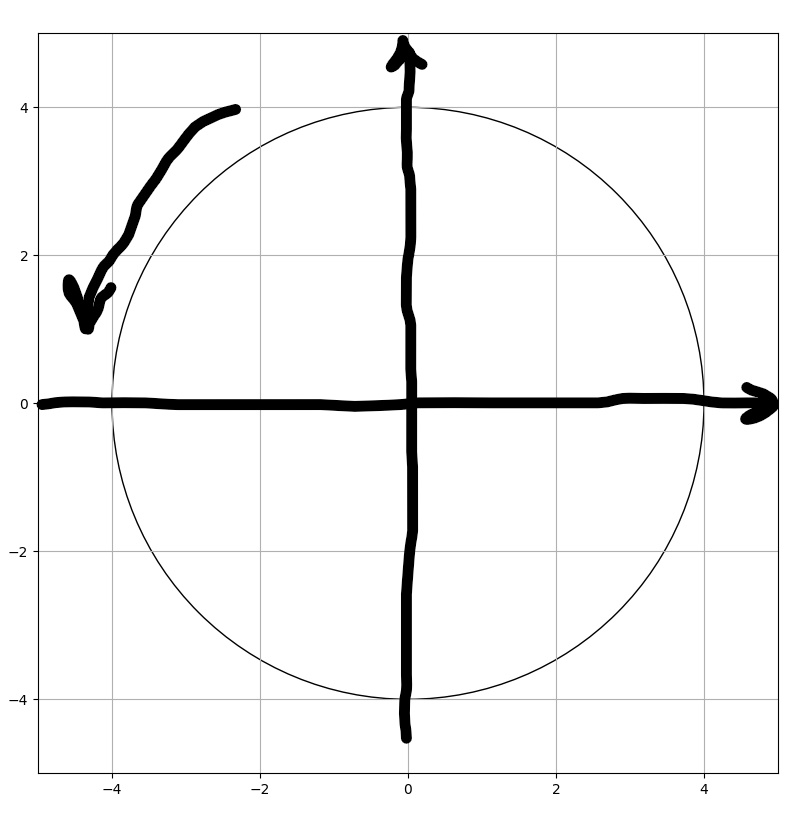
\includegraphics[scale=0.25]{9}
    \end{center}
        
    начиная с \(n > N\ a - \varepsilon < a_n < a + \varepsilon \ \forall \varepsilon\), но тогда \(\forall n_k > N \ a - \varepsilon < a_{nk} < a + \varepsilon \Rightarrow\) т.е. \(\lim_{k \rightarrow \infty}{a_{nk}} = a \ \downarrow\)

    \textbf{Следствие}

    \( x_n = (-1)^n \)

    Если \( \exists\ x_{nk} \textrm{ и } x_{nk}':\ \lim_{k \rightarrow \infty} x_{nk} \neq \lim_{k \rightarrow \infty} x_{nk}' \Rightarrow \not\exists\ \lim x_n \)
    
    \subsection{Теорема Больцано-Вейерштрасса}
    
    Если \( \{x_n\} \) \underline{ограничена}, то \( \exists \)-ет хотя бы одна сходящаяся подпоследовательность.

    \(\uparrow\)
    \begin{enumerate}
        \item Раз ограничена; то \(\exists\ M\ :\ \forall n\ \abs{x_n} \leq M\), т.е. \(I_0 = [-M; M]\), то \(\forall n\ x_n \in I_0\)\\
        \( d_0 = 2M \)

        \item \( \frac{I_0}{2} \) (делим \( I_0 \) пополам)\\
        Пусть \( I_1 \)-та половина, в которой содержится \( \infty \) число членов последовательности \(x_n\) (если в обеих, то выбираем любую из них) \( I_1 = \frac{I_0}{2} \)\\
        \( d_1 = \frac{2M}{2} \)

        \item \( \frac{I_1}{2} \Rightarrow\), та часть, в которой содержится \( \infty \) число членов последовательности \( \{x_n\} \) (если в обеих, то любую из) в \( I_2\ b_2 = x_{n2} \in I_2\ n_2>n_1 \)\\
        \( d_1 = \frac{2M}{2^2} \)
        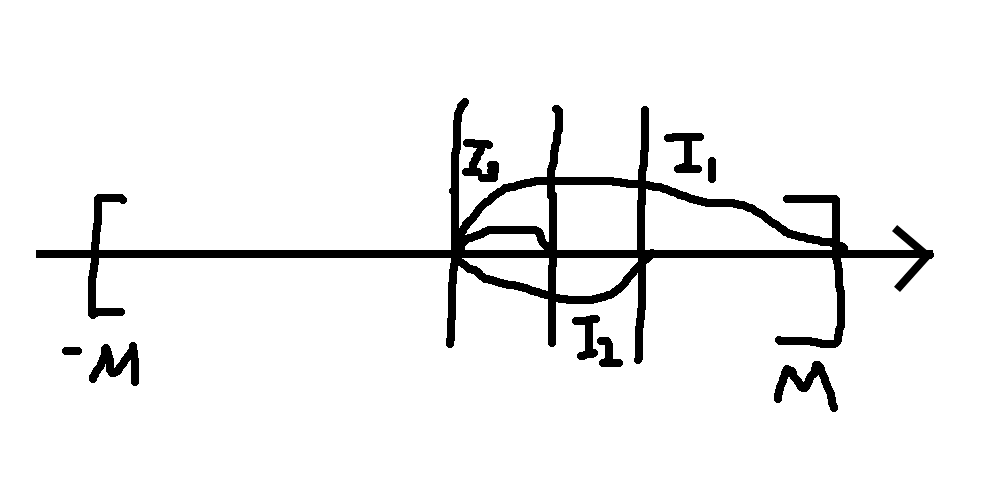
\includegraphics[scale=0.25]{10}
        \item и т.д. \(I_0 \supset I_1 \supset I_2 \supset ... \supset I_k \supset .....\)
        \\k)\(d_k = \frac{2M}{2^k} \longrightarrow_{k \rightarrow \infty} 0\)
    \end{enumerate}
    по Т. о вложенных промежутках \(\exists !\ B\ :\ B \in I_k\ \forall k\)
    \\Покажем, что \(\{b_k\} \xrightarrow[k \rightarrow \infty]{} B\)
    
    \( \forall \varepsilon > 0 \exists\ K: \forall k > K:\) 

    \(\abs{b_k - B} < \varepsilon\)

    \( \abs{b_k - B} < \abs{I_k} = \frac{2M}{2^k} < \frac{2M}{k} < \varepsilon \)

    \( 2^k > k\ K = [\frac{2M}{\varepsilon}] + 1\)

    \(\downarrow\)
    
    \subsection{Определения верхнего и нижнего пределов}
    
    \subsubsection{Верхний предел}
    
    \textbf{Определение.} Число M будем называть верхним пределом последовательности \(x_n\), если
    \begin{enumerate}
        \item \( \exists\ x_{nk}: x_{nk}  \xrightarrow[k \rightarrow \infty]{} M\)
    
        \item \(\forall x'_{nk} \rightarrow M'\ M' \leq M\)

    \end{enumerate}
    \( \uparrow \)

    \textbf{Обозначение.} \(\quad \overline{\lim_{n \rightarrow \infty}}\ x_n = \overline{\lim} x_n = M \)
    
    \textbf{Замечание.} 
    \begin{enumerate}
        \item Если \(x_n\) не ограничена сверху, то \(\overline{\lim}x_n = +\infty\)
        
        \item Если \(\overline{\lim}x_n = a\)(a --- конечное число)
    \end{enumerate}
    
    \subsubsection{Нижний предел}
    
    \textbf{Определение.} Число m будем называть нижним пределом последовательности \(x_n\), если
    \begin{enumerate}
        \item \( \exists\ x_{nk}: x_{nk}  \xrightarrow[k \rightarrow \infty]{} m\)
    
        \item \(\forall x'_{nk} \rightarrow m'\ m' \leq m\)

    \end{enumerate}

    \textbf{Обозначение.} \(\quad \underline{\lim_{n \rightarrow \infty}}\ x_n = \underline{\lim} x_n = M \)

    \textbf{Замечание.} 
    \begin{enumerate}
        \item Если \(x_n\) не ограничена снизу, то \(\underline{\lim}x_n = -\infty\)
        
        \item Если \(\underline{\lim}x_n = a\)(a --- конечное число)
    \end{enumerate}
	
    \subsection{Необходимое и достаточное условие существования предела}
    
    \textbf{Теорема.} \( \exists\ \lim_{n \rightarrow \infty} x_n = A \) (конечн, \(+\infty\), \(-\infty\)) \( \Leftrightarrow \overline{\lim}x_n = \underline{\lim}x_n = A \)

    \(\uparrow\)
    "\(\Rightarrow\)" пусть \(\lim_{n \rightarrow \infty}{x_n} = A\)

    \begin{enumerate}
        \item \( A = +\infty \), т.е. \( lim_{n \rightarrow \infty}x_n = +\infty \)\\
        \( \Rightarrow \underline{lim}x_n = +\infty \Rightarrow \overline{lim}x_n = +\infty \)   
        \item \(A = -\infty\); т.е. \(\lim_{n \rightarrow \infty}{x_n} = -\infty \Rightarrow \overline{\lim}x_n = -\infty \Rightarrow \underline{\lim}x_n = -\infty\)
        \item Если \( \lim_{n \rightarrow \infty}x_n = A \) (A --- конечное число) \( \Rightarrow \overline{\lim}x_n = \underline{\lim}x_n = A \) уже доказывали
    \end{enumerate}

    "\( \Leftarrow \)"
    \begin{enumerate}
        \item \(\lim x_n = +\infty\)
        т.е. \(\lim{n \rightarrow \infty}{x_n} = +\infty\)
        
        \item \( \overline{\lim}x_n = -\infty \)
        \( \Rightarrow \lim x_n = -\infty \)

        \item A --- конечный \(\overline{\lim} x_n = \underline{\lim} x_n = A\)
    \end{enumerate}
    Надо \( \forall \varepsilon > 0\ \exists N\ \forall n > N\ A - \varepsilon <_{\textrm{из } \underline{\lim}x_n = A} x_n <_{\textrm{из } \overline{\lim}x_n = A} A + \varepsilon \), т.е. \( \lim_{n \rightarrow \infty}x_n = A \)
    
    \( \downarrow \)
    
    \subsection{Теорема о существовании верхнего и нижнего предела у произвольной последовательности}
    
    \textbf{Теорема.} У всякой \(\{x_n\}\ \exists\ \overline{\lim}\) и \(\underline{\lim}\).

    \(\uparrow\)
    \begin{enumerate}
        \item \(x_n\) --- не ограничена сверху, то \(\overline{\lim}x_n = +\infty\)
        \item \(x_n\) --- не ограничена снизу, то \(\underline{\lim}x_n = -\infty\)
        \item \(x_n\) ограничена сверху и снизу
    \end{enumerate}

    дальше как в Т. Больцано-Вейерштрасса, только 3.1) если ищем \( \overline{\lim} \), то всегда беру правую половинку, если возникает выбор.
    \\ 3.2) Для \(\underline{\lim}\), то беру левую половинку

    \( \downarrow \)

    \textbf{Замечание.} Очевидно, что \( \underline{\lim}x_n \leq \overline{\lim}x_n\)
    
    \subsection{Фундаментальные последовательности, критерий Коши сходимости последовательности}
    
  	\textbf{Определение.} Последовательность \( x_n \) называется фундаментальной(удовлетворяет условию Коши), если \( \forall \varepsilon > 0\ \exists N: \forall n, m > N,\ \abs{x_n - x_m} < \varepsilon \)
    
    \(x_m - \varepsilon < x_n < x_m + \varepsilon\)

    \textbf{Теорема. Критерий Коши.} Числовая последовательность \( \{x_n\} \) сходится \( \Leftrightarrow \forall \varepsilon > 0\ \exists N(\varepsilon): \forall n, m > N: \abs{x_n - x_m} < \varepsilon \) 

    \(\uparrow\)
    
    "\(\Rightarrow\)" пусть сходится (\(\lim_{n \rightarrow \infty}{x_n} = a\) --- конечное число) \(\forall \varepsilon > 0\ \exists N : \forall n > N: \abs{x_n - a} < \frac{\varepsilon}{2} \)

    \( \abs{x_n - x_m} = \abs{x_n - a + a - x_m} \leq \abs{x_n - a} + \abs{a - x_m} = \abs{x_n - a} + \abs{x_m - a} <_{n > N; m > N} \frac{\varepsilon}{2} + \frac{\varepsilon}{2} = \varepsilon \)

    "\(\Leftarrow\)" 1) покажем, что \(\{x_n\}\) --- ограничена \(\forall \varepsilon > 0\ \exists N_0 : \forall n,m > N_0,\ \abs{x_n - x_m} < \varepsilon\)
    
    Пусть \(\varepsilon = 1\)
    \\\(\abs{x_n} - \abs{x_m} \leq \abs{x_n - x_m} < 1\)
    \\\( \Downarrow \)
    \\\( \abs{x_n} < 1 + \abs{x_m} \)

    Фиксированный \( m \Rightarrow \forall n > N_0 \) рассмотрим \( M = \max{\{ 1 + \abs{x_m}; \abs{x_1}; \abs{x_2}; \abs{x_3}; ... ; \abs{x_{N_0}} \}} \)
    
    2) По Т. Больцано-Вейерштрасса из \(\{x_n\}\) можно выделить сходящиеся последовательности
    \\\(\exists x_{nk}\ :\ x_{nk} \xrightarrow[k \rightarrow \infty]{} a \)
    
	Покажем, что \( x_n \rightarrow a \), т.е. \(\forall \varepsilon > 0\ \exists N_0\ :\ \forall n, m > N_0,\ \abs{x_n - x_m} < \varepsilon \)

    Имеем:\\
    \(\forall \varepsilon > 0\ \exists N_0\ :\ \forall n, m > N_0,\ \abs{x_n - x_m} < \frac{\varepsilon}{2}\) и\\
    \(x_{nk} \rightarrow a\), т.е. \(\forall \varepsilon > 0\ \exists K_0\ :\ \forall k > K_0,\ \abs{x_{nk} - a} < \frac{\varepsilon}{2}\)

    \(\abs{x_n - a} = \abs{x_n - x_{nk} + x_{nk} - a} \leq \abs{x_n - x_{nk}} + \abs{x_{nk} - a} < \frac{\varepsilon}{2} + \frac{\varepsilon}{2} = \varepsilon\)
    \\ \(n_k > N_0\\ k > K_0\ n_k > n_{K_0}\)
    \\\(N = \max(N_0, n_{K_0})\)
    \\\(\downarrow\)
    
\end{document}
